\chapter{Experimentos}
\label{cap:capitulo6}

En este capítulo se recogen las distintos experimentos que se han llevado a cabo durante el desarrollo del proyecto. Estas pruebas han sido fundamentales para verificar el correcto funcionamiento del sistema de reconocimiento de maduración de frutos y su comunicación con el brazo robótico, permitiendo así alcanzar los objetivos definidos en fases anteriores del trabajo.

\section{Detección con YOLOv3 y TensorFlow}
\label{exp_seleccion_algoritmo}

Dada la finalidad del proyecto, se requería que la detección de objetos se diera en tiempo real, por lo que se buscó información sobre YOLO, un sistema de código abierto que permitía esto a partir de una red neuronal convolucional para detectar objetos en imágenes y vídeo, y se iniciaron las pruebas pertinentes para la selección del algoritmo de detección y de las bibliotecas a utilizar.

\subsection{Pruebas con imágenes}
\label{sec:Pruebas_imgs_TF}

En primer lugar, se creó un entorno de Anaconda para poder probar la detección de objetos en imágenes utilizando Tensorflow mediante el repositorio \textit{deteccion\_objetos}\footnote{\url{https://github.com/puigalex/deteccion_objetos}} basados en la configuración \textit{faster rcnn resnet101 coco} de los modelos de detección de objetos de Tensorflow para poder llevar a cabo la comparación, y etiquetando imágenes, en este caso de tigres, mediante la herramienta labelImg\footnote{\url{https://github.com/HumanSignal/labelImg}}, se prepararon las carpetas y archivos de configuración correspondientes para poder llevar a cabo el entrenamiento del modelo siguiendo los pasos indicados en el repositorio utilizando una distribución de las imágenes utilizadas para el aprendizaje del modelo y su uso en la detecciónn aproximadamente del 70:30 (73\% datos de entrenamiento y 27\% datos de prueba)(Cuadro \ref{tab:Imagenes_Entrenamiento}), a partir de los cuales se entrenó ese 70\% con uno de los algoritmos y los respectivos parámetros escogidos y medimos su rendimiento usando el 30\% restante de los datos.

  \begin{table}[H]
  \centering
  \begin{tabularx}{\textwidth}{|X|X|X|}
    \hline
    \centering \textbf{Imágenes usadas en entrenamiento} & 
    \centering \textbf{Imágenes usadas en test} & 
    \centering \textbf{Número total de imágenes} \tabularnewline
    \hline
    \centering 594 & \centering 218 & \centering 812 \tabularnewline
    \hline
  \end{tabularx}
  \caption{Distribución de las imágenes utilizadas para el entrenamiento del modelo}
  \label{tab:Imagenes_Entrenamiento}
  \end{table}

Se entrenó este modelo hasta que se observó que la pérdida estaba por debajo de 1, considerando que esta pérdida no era alta, y que no existían demasiadas fluctuaciones,  deteniendo este entrenamiento a los 1400 pasos, a pesar de que este entrenamiento estuviera programado para llegar hasta los 20000, ya que se trataba de una prueba simplemente. Esto supuso que se tuviera que utilizar el último checkpoint disponible, en este caso el del paso 1337 (Figura \ref{fig:Deteccion_Prueba_TF}), para convertirlo en un modelo final y de esta manera poder generar predicciones, utilizando imágenes de diferentes tamaños.

  \begin{figure}[H]
    \begin{center}
      \subcapcentertrue
      \subfigure[Pasos finales del entrenamiento con TensorFlow]{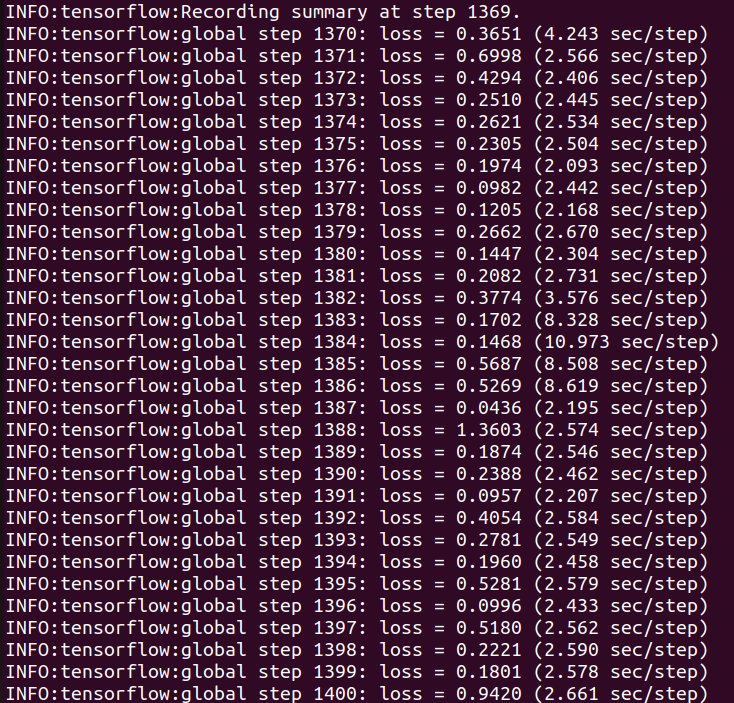
\includegraphics[height=50mm, width=70mm]{figs/Pasos finales del entrenamiento_TF.png}}
      \hspace{4mm}
      \subfigure[Checkpoints del entrenamiento con TensorFlow]{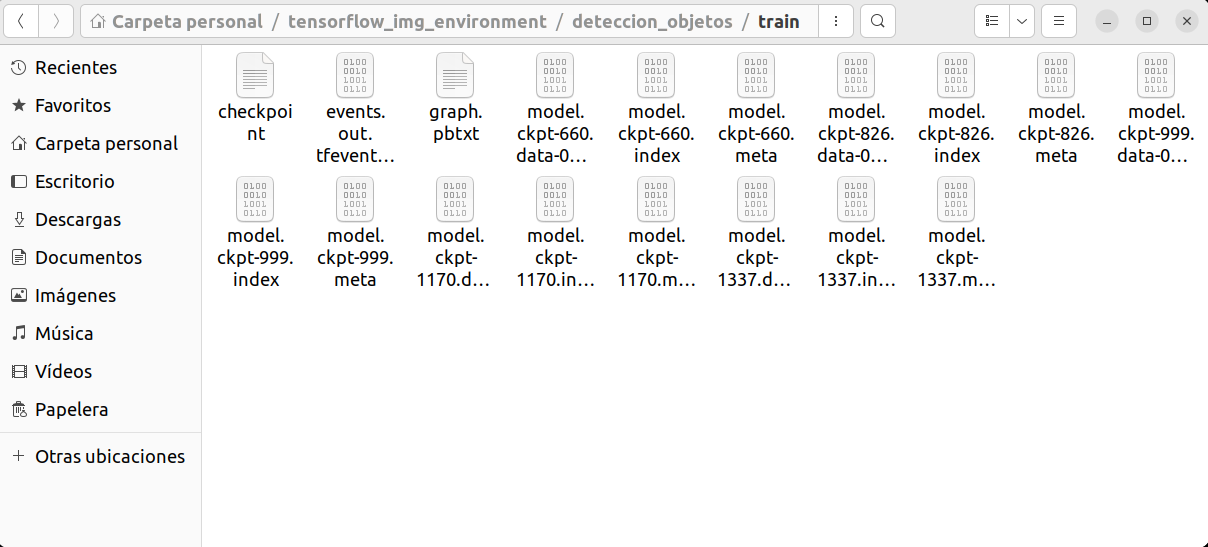
\includegraphics[height=50mm, width=70mm]{figs/checkpoints_TF.png}}
    \end{center}
    \caption{Entrenamiento del algoritmo con TensorFlow}
    \label{fig:Deteccion_Prueba_TF}
  \end{figure}
  
Una vez convertido el checkpoint en un modelo final, se procedió a realizar las primeras pruebas de detección en imágenes de este modelo, comprobando su capacidad para detectar correctamente los tigres para este caso, y evaluar visualmente los resultados obtenidos en algunos ejemplos mostrados en la Figura \ref{fig:deteccion_tensorflow_tigres}, de estas primeras detecciones realizadas tras el entrenamiento.

  \begin{figure}[H]
  \centering
  % Fila 1
  \begin{minipage}{0.46\textwidth}
    \centering
    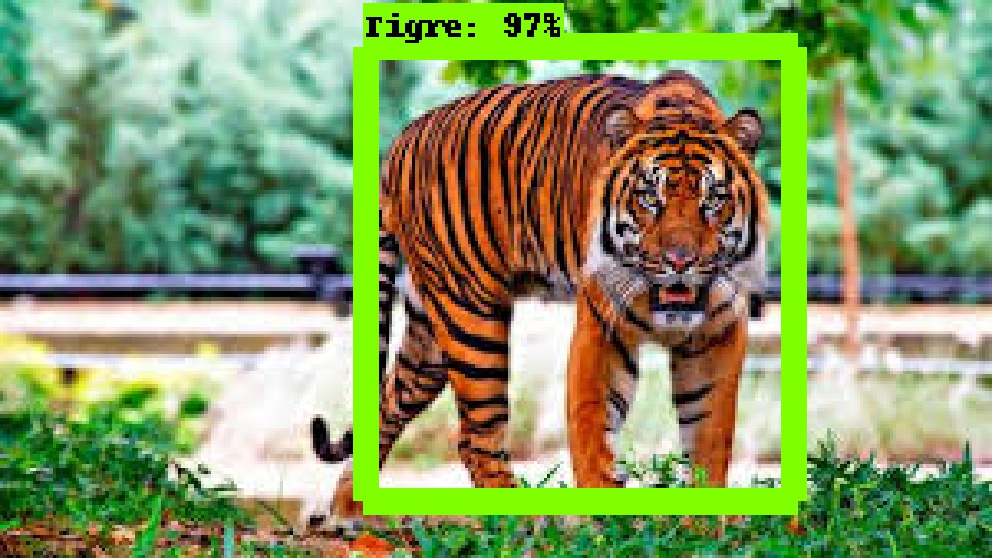
\includegraphics[width=\linewidth]{figs/tigre_1.jpeg}
  \end{minipage}
  \hspace{2mm}
  \begin{minipage}{0.46\textwidth}
    \centering
    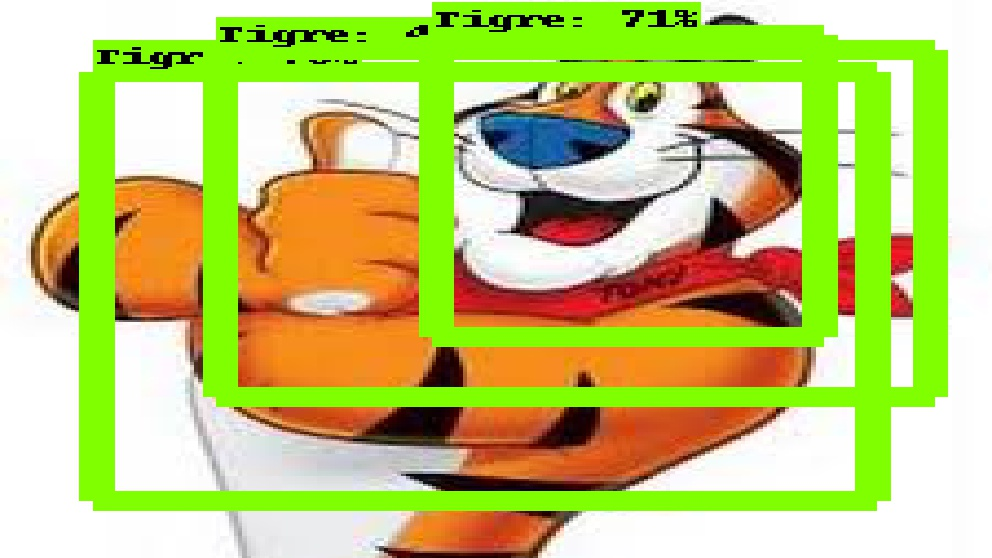
\includegraphics[width=\linewidth]{figs/tigre_2.jpeg}
  \end{minipage}
  \\[4mm] % Espacio vertical entre las dos filas
  % Fila 2
  \begin{minipage}{0.46\textwidth}
    \centering
    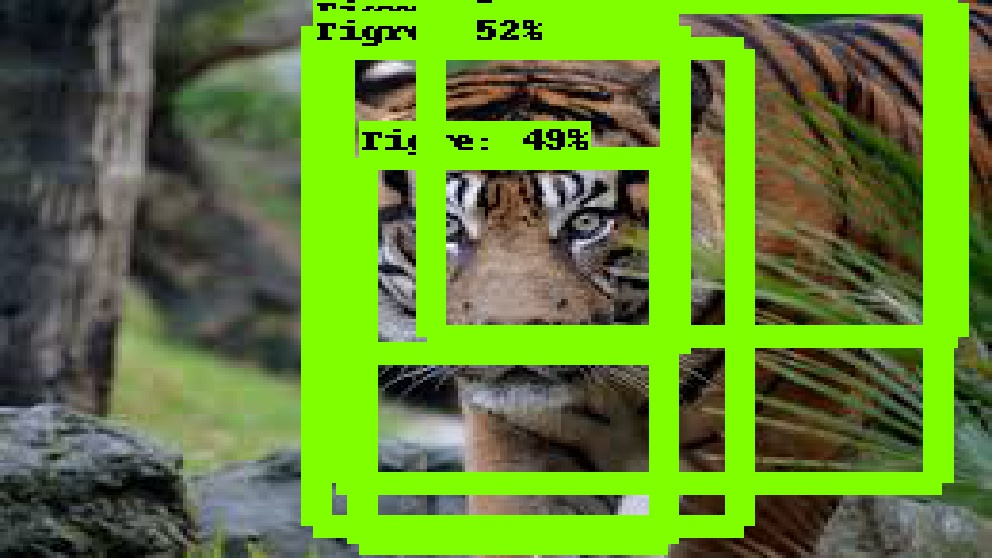
\includegraphics[width=\linewidth]{figs/tigre_4.jpeg}
  \end{minipage}
  \hspace{2mm}
  \begin{minipage}{0.46\textwidth}
    \centering
    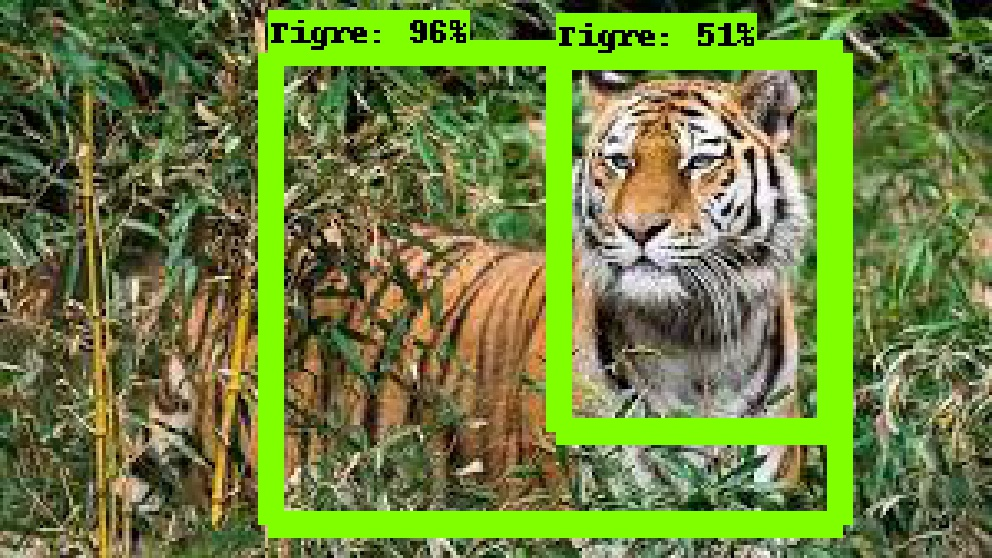
\includegraphics[width=\linewidth]{figs/tigre_5.jpeg}
  \end{minipage}
  \caption{Resultado de la detección en imágenes con TensorFlow}
  \label{fig:deteccion_tensorflow_tigres}
  \end{figure}
 
Dados los resultados obtenidos en las imágenes utilizadas para esta primera prueba, se decidió llevar a cabo un nuevo proceso de entrenamiento a partir del último checkpoint disponible con el objetivo principal de comprobar si, aumentando el número de pasos de entrenamiento, se lograba una mejora significativa tanto en la disminución del valor de pérdida como en el incremento del porcentaje de confianza en las detecciones realizadas. Así, se retomó el entrenamiento desde el checkpoint del paso 1337, extendiéndose en esta segunda ocasión hasta el paso 2945, momento en el cual se optó por detener manualmente el proceso al observarse una estabilización progresiva en los valores de pérdida, y siendo este último checkpoint generado fue el correspondiente al paso 2877, obteniéndose en este punto un valor de pérdida de tan solo 0.222, notablemente inferior al registrado en el primer intento. A continuación, se procedió a ejecutar nuevamente el programa sobre las mismas imágenes de prueba de tigres empleadas en la primera serie de tests, lo que permitió realizar una comparación directa entre ambos modelos, y observar que en esta segunda ejecución existía una clara mejora en la calidad de las detecciones, tanto en términos de mayor porcentaje de confianza como en la precisión de los cuadros delimitadores sobre los objetos detectados (ver Figura \ref{fig:deteccion_tensorflow_tigres_v2}).

  \begin{figure}[H]
  \centering
  % Fila 1
  \begin{minipage}{0.46\textwidth}
    \centering
    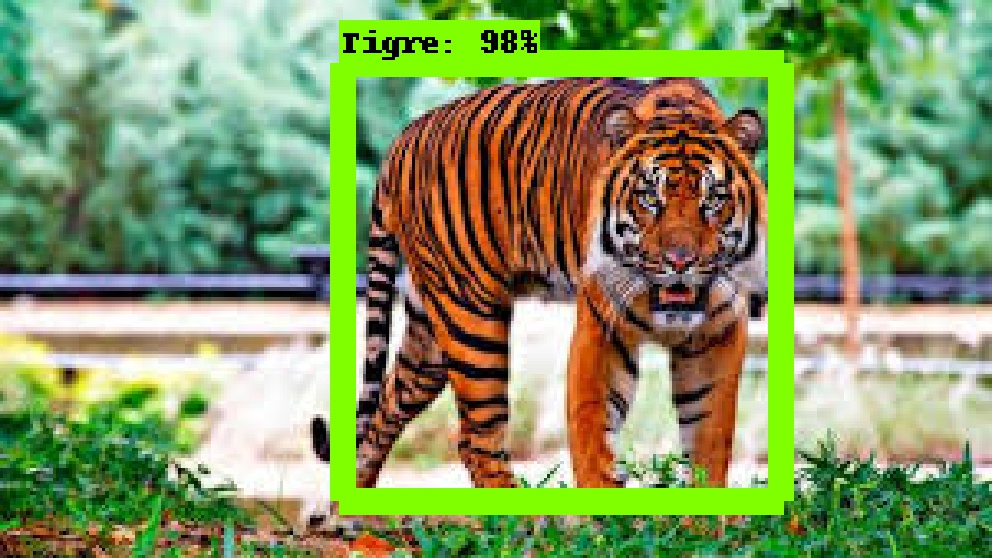
\includegraphics[width=\linewidth]{figs/tigre_1_v2.jpeg}
  \end{minipage}
  \hspace{2mm}
  \begin{minipage}{0.46\textwidth}
    \centering
    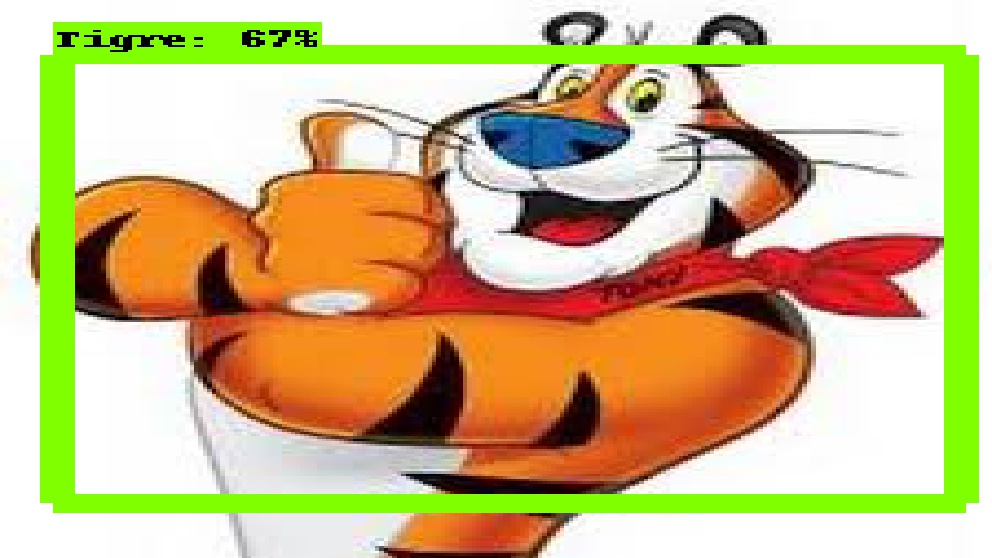
\includegraphics[width=\linewidth]{figs/tigre_2_v2.jpeg}
  \end{minipage}
  \\[4mm] % Espacio vertical entre las dos filas
  % Fila 2
  \begin{minipage}{0.46\textwidth}
    \centering
    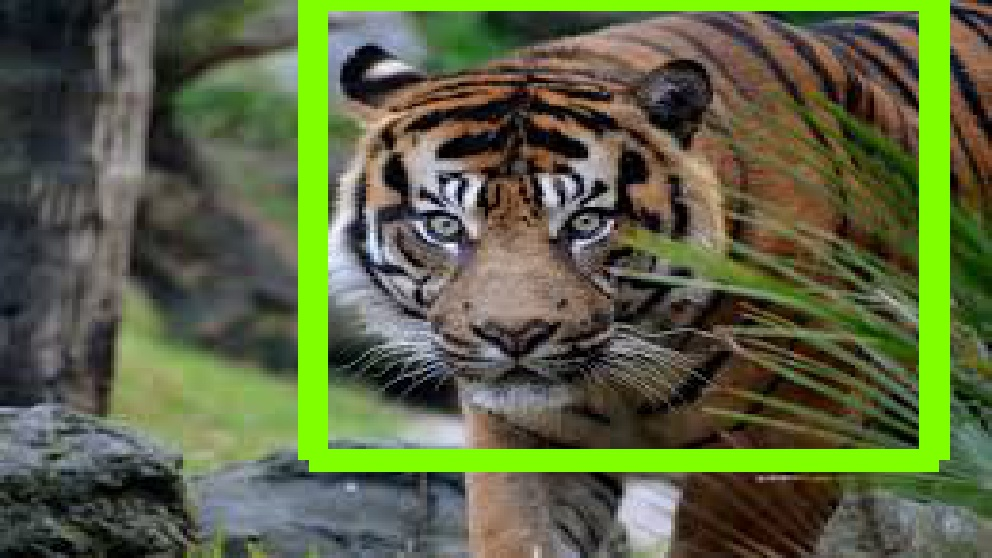
\includegraphics[width=\linewidth]{figs/tigre_4_v2.jpeg}
  \end{minipage}
  \hspace{2mm}
  \begin{minipage}{0.46\textwidth}
    \centering
    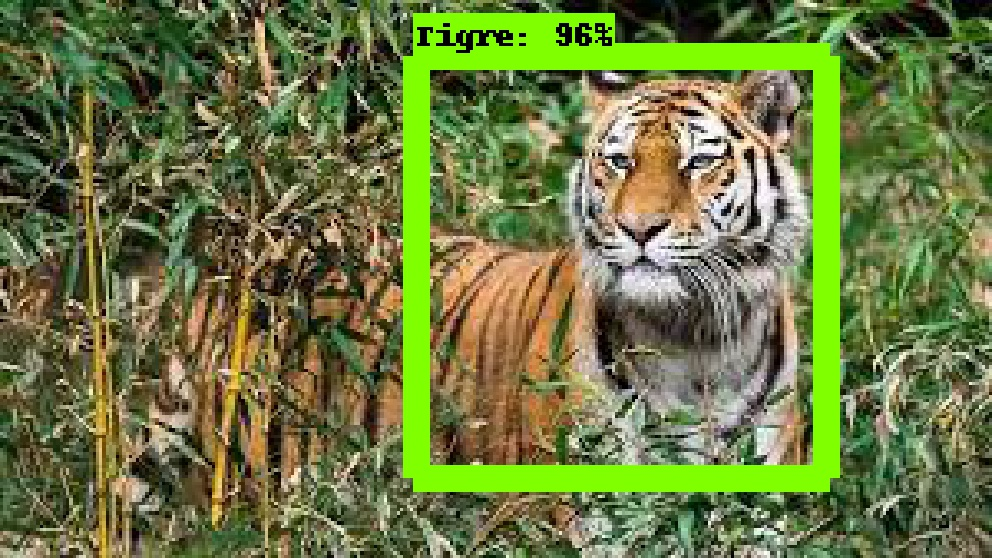
\includegraphics[width=\linewidth]{figs/tigre_5_v2.jpeg}
  \end{minipage}
  \caption{Resultado del reentrenamiento de la detección en imágenes con TensorFlow}
  \label{fig:deteccion_tensorflow_tigres_v2}
  \end{figure}


Después de llevar a cabo estas poruebas con el ejemplo de los tigres, se comprobó si el modelo funcionaría también con el objeto final, en este caso, con fresas, por lo que, a través de la página Kaggle, se obtuvo un dataset de 262 frutas\footnote{\url{https://www.kaggle.com/datasets/aelchimminut/fruits262}} de las cuales únicamente se utilizó el archivo de las fresas, que contenía 1002 imágenes para llevar a cabo estas pruebas.\\

Una vez descargado el archivo, se comenzó a etiquetar una a una las imágenes mediante la herramienta labelImg para obtener los archivos xml, tal y como se había hecho con el ejemplo anterior de los tigres, y antes de terminar de etiquetar el dataset entero, se probó este modelo utlizando las primeras 405 imágenes etiquetadas siguiendo una distribución de estas del 80:20 para su entrenamiento y usando el checkpoint guardado en el paso 3490 para congelar el modelo, y así poder utilizar varias imágenes aún por etiquetar para probarlo, obteniendo un resultado satisfactorio en cuanto a la detección y su confianza, tal y como se puede observar en la Figura \ref{fig:Deteccion_Fresas_Imagenes_TF}.

  \begin{figure}[H]
  \centering
  % Fila 1
  \begin{minipage}{0.45\textwidth}
    \centering
    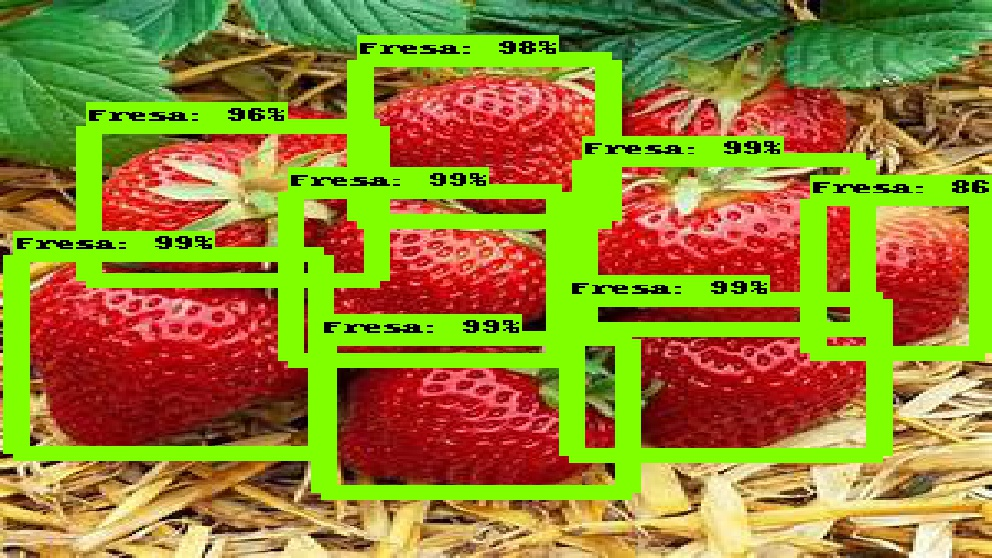
\includegraphics[width=\linewidth]{figs/999.jpeg}
  \end{minipage}
  \hspace{2mm}
  \begin{minipage}{0.45\textwidth}
    \centering
    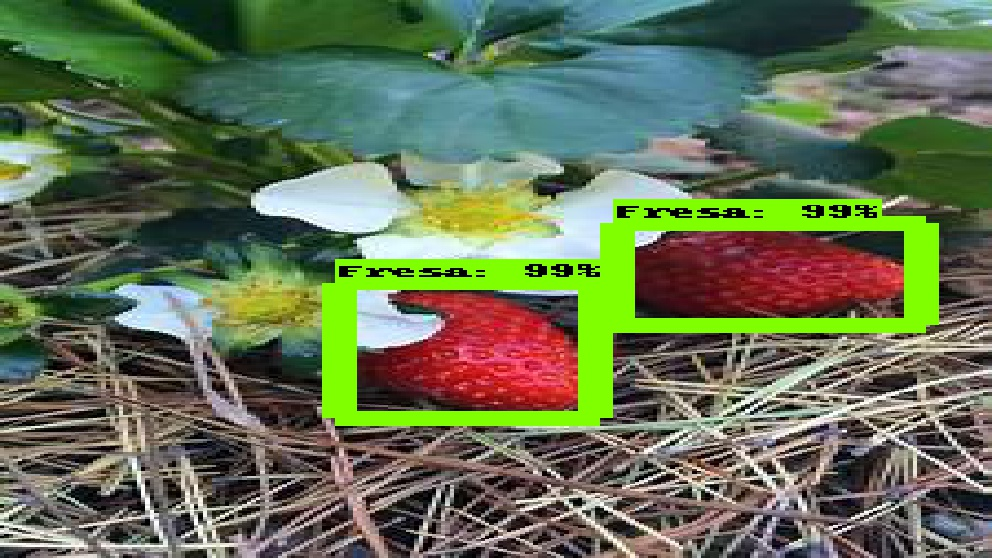
\includegraphics[width=\linewidth]{figs/947.jpeg}
  \end{minipage}
  \\[4mm] % Espacio vertical entre las dos filas
  % Fila 2
  \begin{minipage}{0.45\textwidth}
    \centering
    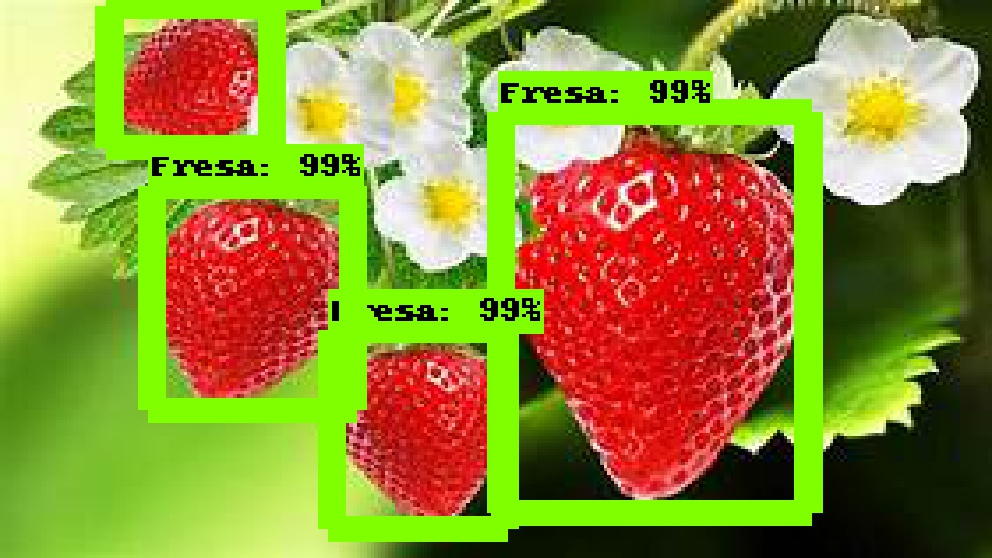
\includegraphics[width=\linewidth]{figs/868.jpeg}
  \end{minipage}
  \hspace{2mm}
  \begin{minipage}{0.45\textwidth}
    \centering
    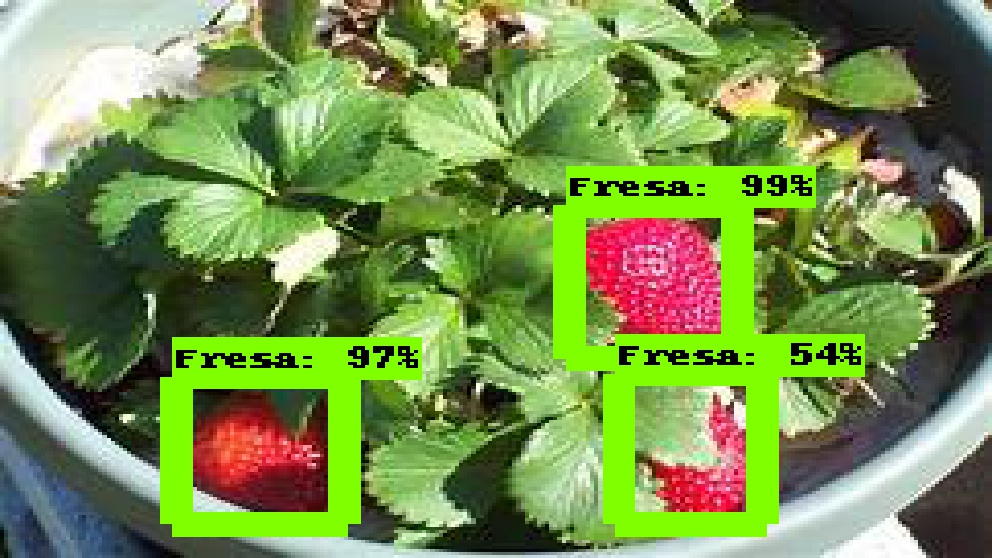
\includegraphics[width=\linewidth]{figs/1000.jpeg}
  \end{minipage}
  \caption{Pruebas de deteccion de fresas en imágenes con TensorFlow}
  \label{fig:Deteccion_Fresas_Imagenes_TF}
  \end{figure}

Tras haber conseguido la detección de fresas en imágenes estáticas utilizando TensorFlow, el siguiente paso dentro del desarrollo del sistema consistió en extender las pruebas a la detección en vídeo en tiempo real, por lo que, de forma análoga a como se había realizado previamente con la librería PyTorch, se procedió a evaluar distintos modelos de detección de objetos pertenecientes al zoo de TensorFlow (TensorFlow 2 Detection Model Zoo), los cuales, al estar ya preentrenados sobre conjuntos de datos de referencia, permitieron llevar a cabo una comparación de estos diferentes modelos o sistemas bajo las mismas condiciones iniciales sin necesidad de realizar un nuevo entrenamiento desde cero. 

\subsection{Pruebas con vídeo en tiempo real}
\label{sec:Pruebas_video_TF}

Para la realización de estas pruebas, se utilizó tanto la cámara web integrada del ordenador portátil como una imagen previamente seleccionada, para que, de esta manera pudieran observarse las diferencias entre los modelos tanto en la detección en vídeo como en la detección en imágenes, y poder valorar qué modelo de los tres distintos probados ofrecería mejores prestaciones en términos de precisión, velocidad de procesamiento y robustez frente a las condiciones reales de trabajo (ver Figuras  \ref{fig:modelo_ssd_mobilenet}, \ref{fig:modelo_efficientdet_d4} y \ref{fig:modelo_faster_rcnn_resnet50}). 

	\begin{figure}[H]
    		\begin{center}
      		\subcapcentertrue
      		\subfigure[Resultado del modelo en imagen]{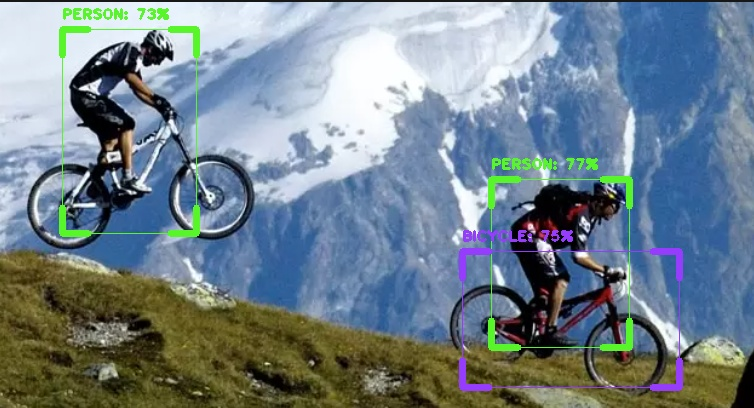
\includegraphics[height=50mm, width=70mm]{figs/ssd_mobilenet_v2_320x320_coco17_tpu-8.jpeg}}
      		\hspace{2mm}
      		\subfigure[Resultado del modelo en vídeo]{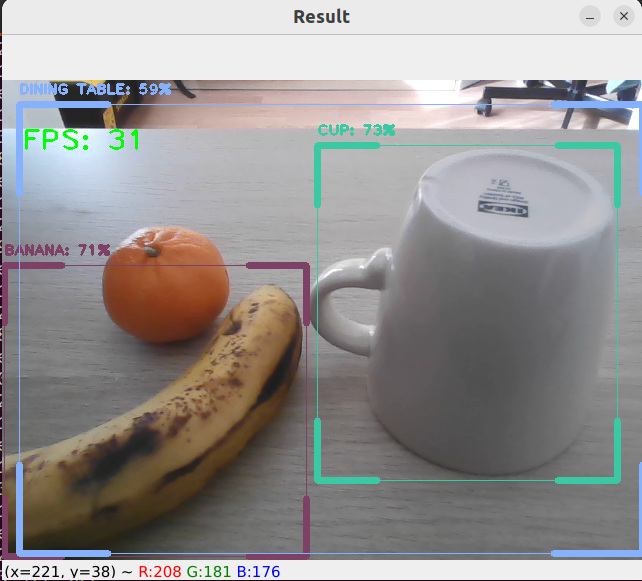
\includegraphics[height=50mm, width=70mm]{figs/webcam ssd_mobilenet_v2_320x320_coco17_tpu-8.png}}
    	\end{center}
    	\caption{Modelo ssd\_mobilenet\_v2\_320x320\_coco17\_tpu-8}
    	\label{fig:modelo_ssd_mobilenet}
  	\end{figure}
  	

  	\begin{figure}[H]
    		\begin{center}
      		\subcapcentertrue
      		\subfigure[Resultado del modelo en imagen]{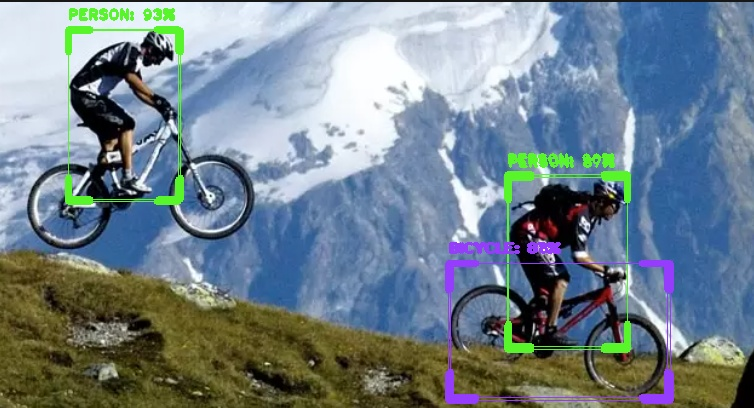
\includegraphics[height=50mm, width=70mm]{figs/efficientdet_d4_coco17_tpu-32.jpeg}}
      		\hspace{2mm}
      		\subfigure[Resultado del modelo en vídeo]{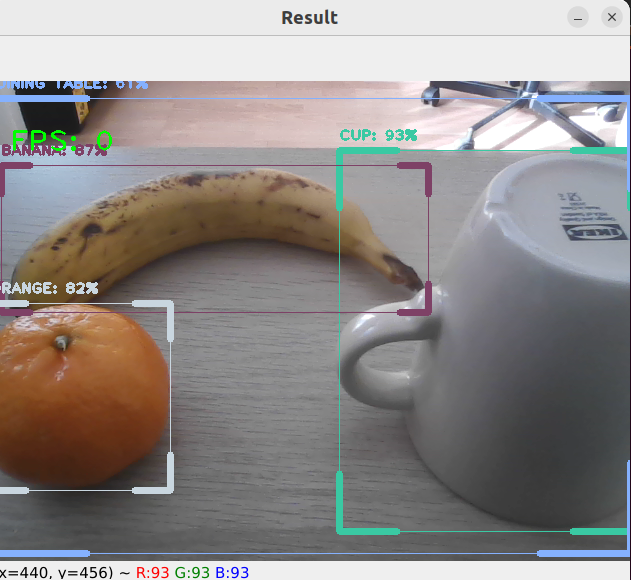
\includegraphics[height=50mm, width=70mm]{figs/webcam efficientdet_d4_coco17_tpu-32.png}}
    	\end{center}
    	\caption{Modelo efficientdet\_d4\_coco17\_tpu-32}
    	\label{fig:modelo_efficientdet_d4}
  	\end{figure}

  	\begin{figure}[H]
    		\begin{center}
      		\subcapcentertrue
      		\subfigure[Resultado del modelo en imagen]{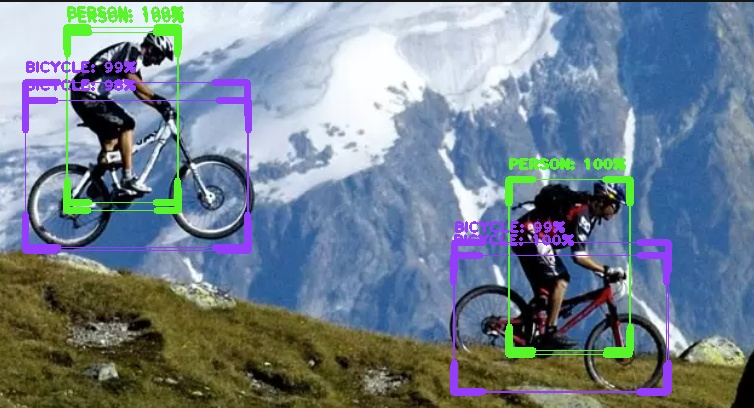
\includegraphics[height=50mm, width=70mm]{figs/faster_rcnn_resnet50_v1_640x640_coco17_tpu-8.jpeg}}
      		\hspace{2mm}
      		\subfigure[Resultado del modelo en vídeo]{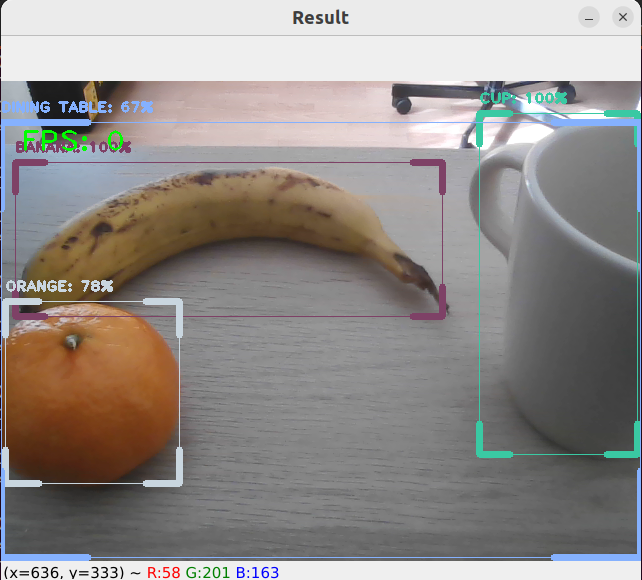
\includegraphics[height=50mm, width=70mm]{figs/webcam faster_rcnn_resnet50_v1_640x640_coco17_tpu-8.png}}
    	\end{center}
    	\caption{Modelo faster\_rcnn\_resnet50\_v1\_640x640\_coco17\_tpu-8 }
    	\label{fig:modelo_faster_rcnn_resnet50}
  	\end{figure}	
  	
\pagebreak

Después de haber llevado a cabo estas pruebas con los modelos de detección de objetos ssd\_mobilenet\_v2\_320x320\_coco17\_tpu-8, efficientdet\_d4\_coco17\_tpu-32 y faster\_rcnn\_resnet50\_v1\_640x640\_coco17\_tpu-8, y tras valorar que, el principal uso del modelo en la aplicación final sería la de llevar a cabo detecciones a tiempo real con una cámara, se escogió el modelo ssd\_mobilenet\_v2 para proseguir con los experimentos, incluso por delante de cualquiera de los otros dos modelos, ya que, a pesar de tener menor precisión y calidad de detección, destacaba principalmente por su elevada velocidad de procesamiento y su bajo consumo de recursos, gracias a su arquitectura ligera basada en MobileNetV2 y su tamaño de entrada reducido, haciéndolo especialmente adecuado para aplicaciones en tiempo real sobre hardware con capacidades limitadas, como puede ser un sistema de visión embarcado en un brazo robótico.\\

Para ello, y dado que para poder llevar a cabo la detección de fresas era necesario utilizar un modelo entrenado desde cero, para lo que se utilizó de guía el repositorio \textit{real\_time\_object\_detection\_cpu}\footnote{\url{https://github.com/haroonshakeel/real_time_object_detection_cpu/blob/main}}, creando y activando un nuevo entorno de Anaconda, donde se instalaron los paquetes y librerías necesarios para ello junto al Object Detection API de TensorFlow junto con Jupyter Notebook\footnote{\url{https://jupyter.org}}, un entorno computacional interactivo basado en web para crear cuadernos que contienen código en vivo, ecuaciones, visualizaciones y texto narrativo. \\

Completada la configuración del entorno, la instalación de todos los componentes, y el entrenamiento del modelo, se realizó una primera prueba de detección utilizando el modelo entrenado para comprobar si funcionaba, obteniendo las primeras predicciones en tiempo real sobre vídeo con fresas reales, y de este modo, poder llevar a cabo la batería de pruebas en las cuales se variaba tanto el número de fresas como las condiciones de luz, siendo los resultados de estos escenarios los que se muestran a continuación en la Figura \ref{fig:deteccion_Fresas_webcam_TF_ssdmobilenet}:
\pagebreak


\begin{figure}[H]
    \centering
    \subcapcentertrue
    % Fila 1
    \subfigure[Una única fresa con luz natural de día]{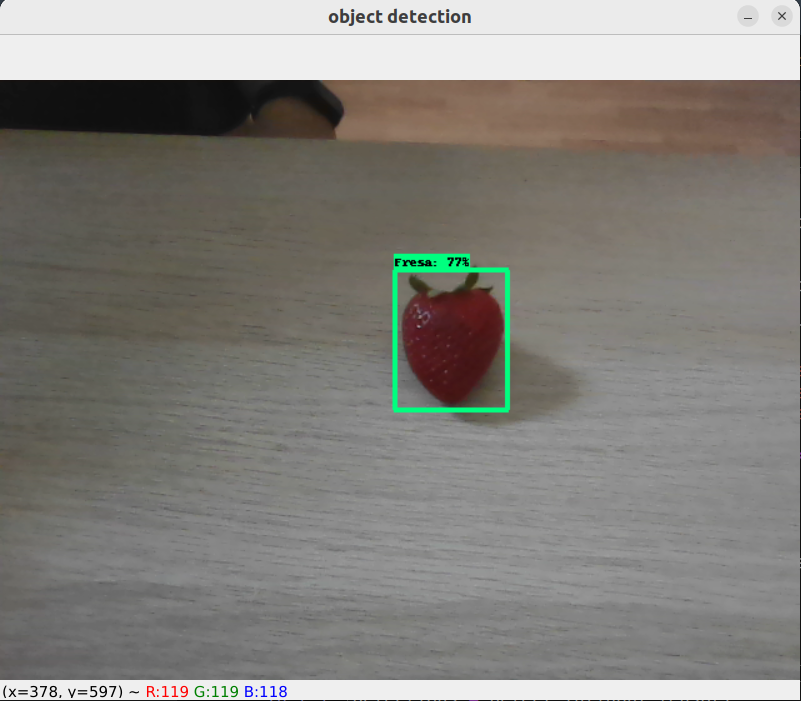
\includegraphics[width=0.30\textwidth]{figs/Deteccion una fresa luz natural dia JN.png}}
    \hspace{1mm}
    \subfigure[Una única fresa con luz artificial de día]{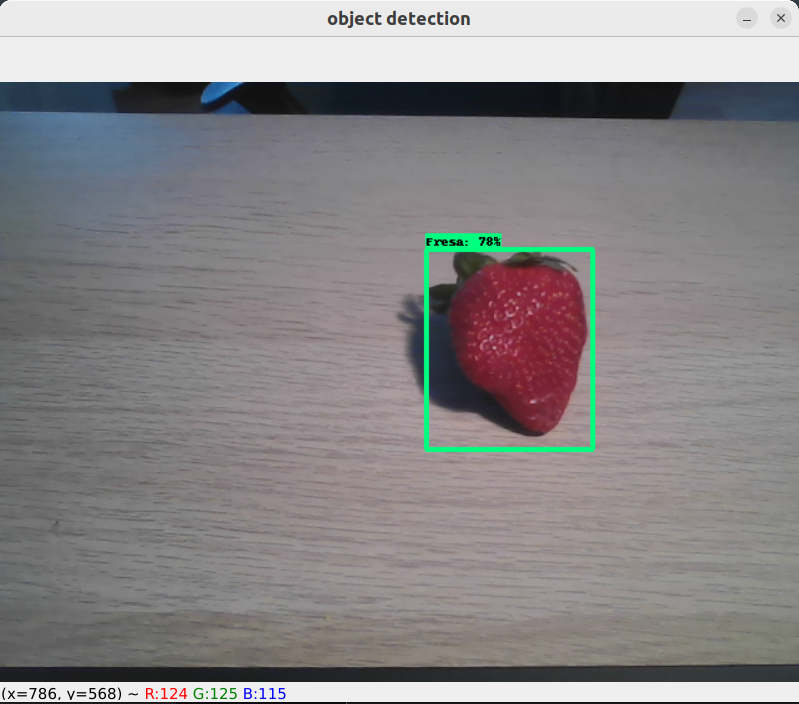
\includegraphics[width=0.30\textwidth]{figs/Deteccion una fresa luz artificial dia JN.png}}
    \hspace{1mm}
    \subfigure[Una única fresa con luz artificial de noche]{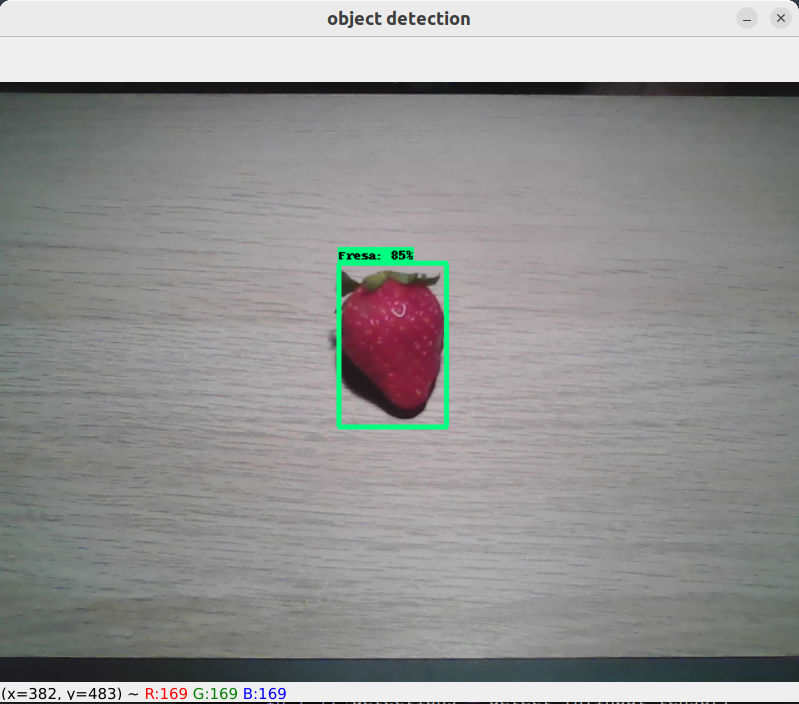
\includegraphics[width=0.30\textwidth]{figs/Deteccion una fresa luz artificial de noche JN.png}}

    \vspace{1mm} % Espacio vertical entre filas

    % Fila 2
    \subfigure[Varias fresas con luz natural de día]{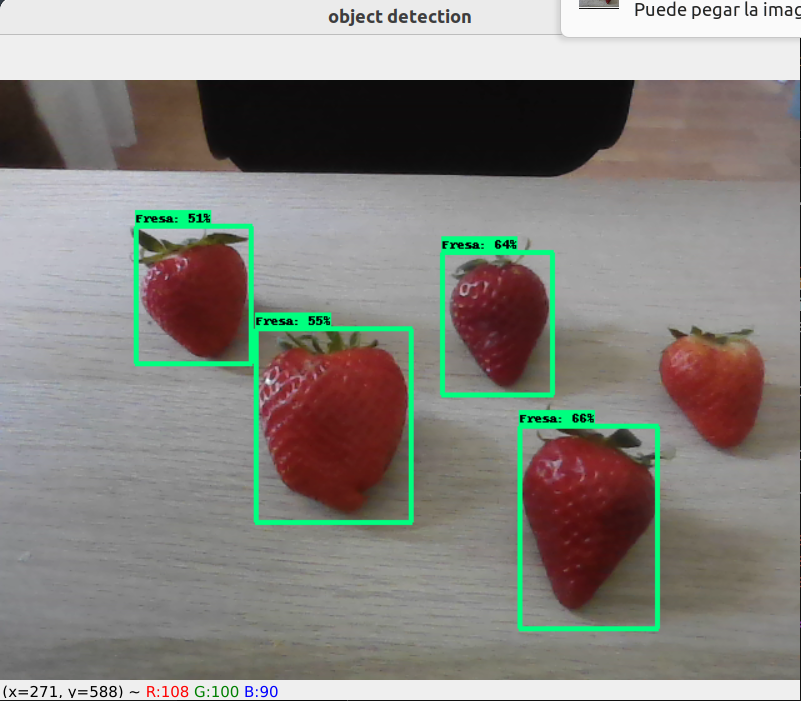
\includegraphics[width=0.30\textwidth]{figs/Deteccion varias fresas luz natural dia JN.png}}
    \hspace{1mm}
    \subfigure[Varias fresas con luz artificial de día]{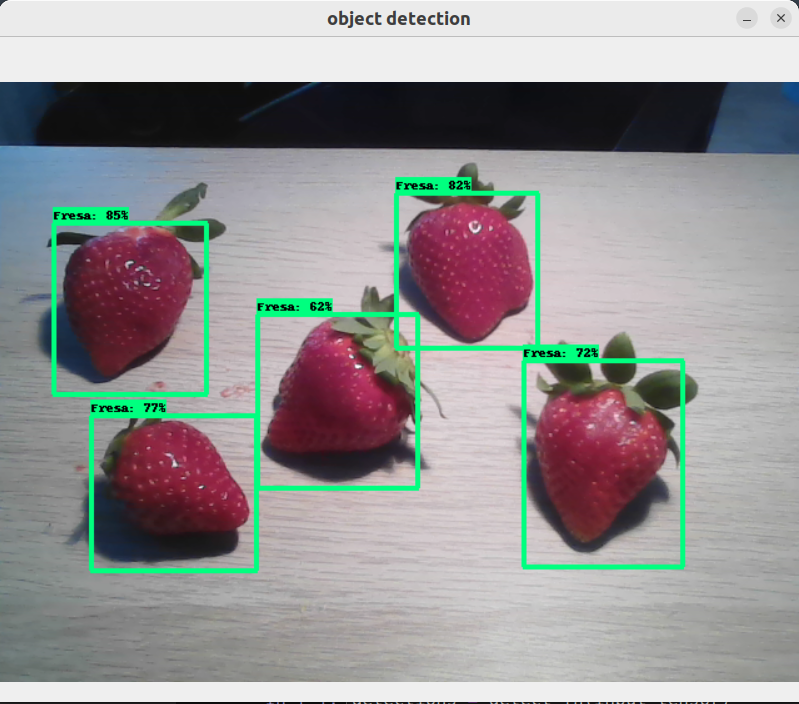
\includegraphics[width=0.30\textwidth]{figs/Deteccion varias fresas luz artificial dia JN.png}}
    \hspace{1mm}
    \subfigure[Varias fresas con luz artificial de noche]{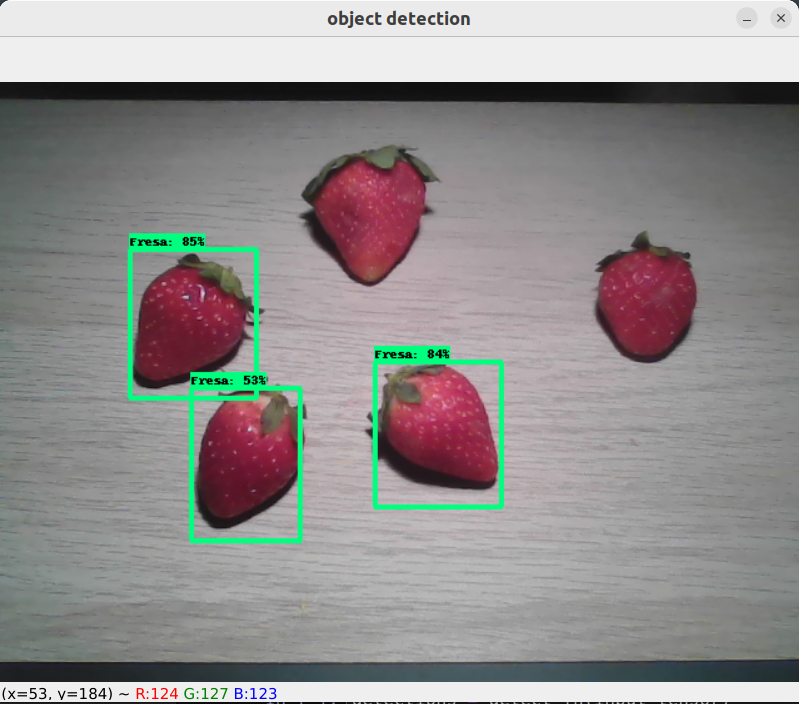
\includegraphics[width=0.30\textwidth]{figs/Deteccion varias fresas luz artificial de noche JN.png}}
    
    \caption{Detección de fresas en webcam con TensorFlow con modelos no pre-entrenados (ssd mobilenet v2 320x320)}
    \label{fig:deteccion_Fresas_webcam_TF_ssdmobilenet}
\end{figure}

Después de verificar la viabilidad y funcionamiento de estas pruebas, y de detectar en los resultados de estas que, con luz artificial en condiciones de alta luminosidad existía un mayor porcentaje de confianza en las detecciones que con luz natural y baja luminosidad, tal y como se puede apreciar en las Figuras \ref{fig:Pruebas_luminosidad} y \ref{fig:Grafica_medias_luminosidad}, se modificó el programa de detección para obtener más datos sobre estas detecciones y para poder mejorar el programa.

    \begin{figure}[H]
    \begin{center}
      \subcapcentertrue
      \subfigure[Resultados de las pruebas de detección con alta luminosidad]{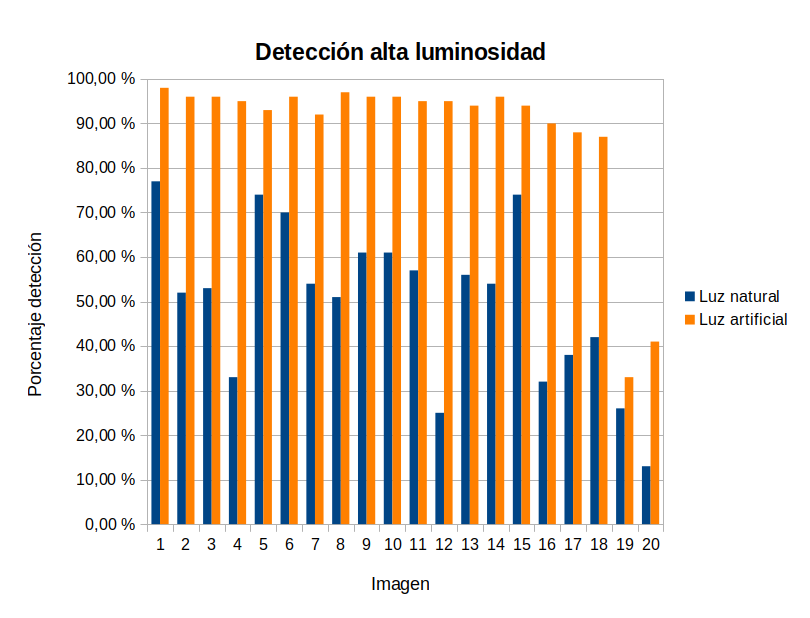
\includegraphics[width=72mm]{figs/Grafica deteccion alta luminosidad.png}}
      \hspace{4mm}
      \subfigure[Resultados de las pruebas de detección con baja luminosidad]{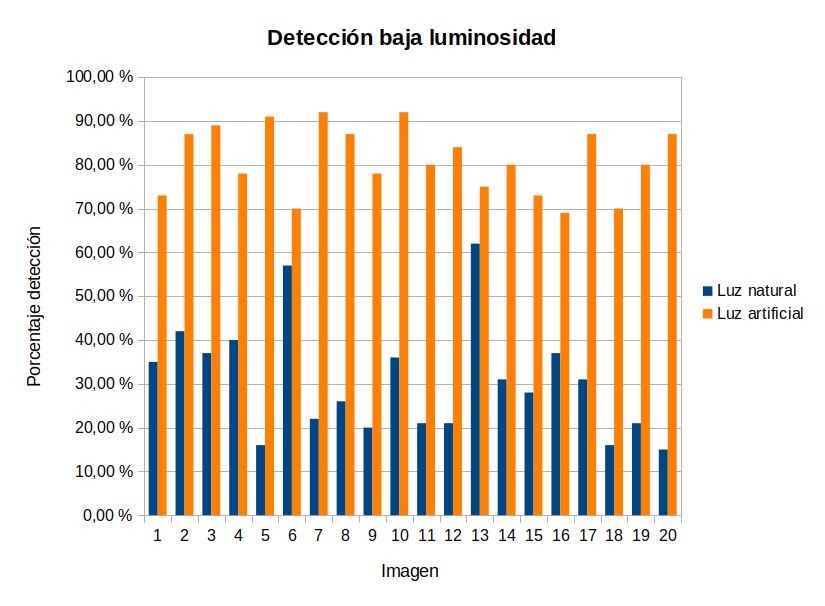
\includegraphics[width=72mm]{figs/Grafica deteccion baja luminosidad.png}}
    \end{center}
    \caption{Gráficas de la confianza de detección obtenida en las pruebas según la luminosidad para el modelo ssd mobilenet v2}
    \label{fig:Pruebas_luminosidad}
  \end{figure}
  
  \begin{figure}[H]
    \begin{center}
      \subcapcentertrue
      \subfigure[Porcentaje medio de confianza para las detecciones con alta luminosidad]{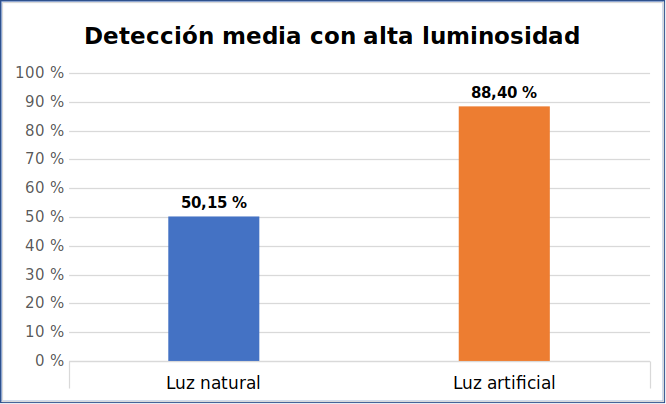
\includegraphics[width=70mm]{figs/Deteccion media con alta luminosidad.png}}
      \hspace{4mm}
      \subfigure[Porcentaje medio de confianza para las detecciones con baja luminosidad]{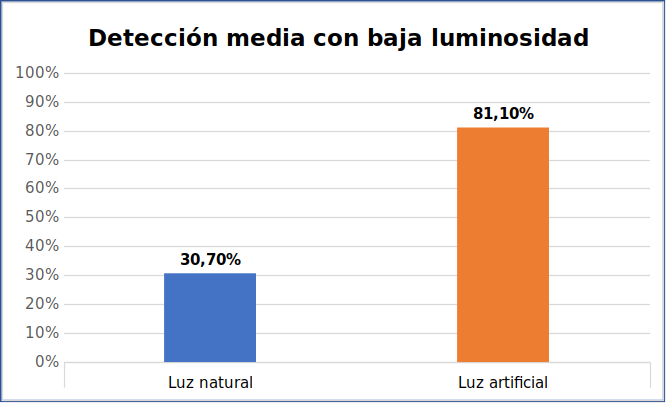
\includegraphics[width=70mm]{figs/Deteccion media con baja luminosidad.png}}
    \end{center}
    \caption{Gráficas de la media de los porcentajes de confianza obtenidos en las pruebas de detección según la luminosidad para el modelo ssd mobilenet v2}
    \label{fig:Grafica_medias_luminosidad}
  \end{figure}


Estas modificaciones incluían la instrucción mediante la cual se dejase de captar lo que se podía ver por la cámara del ordenador y se cerrase la ventana emergente correspondiente, a la que también se le cambió el nombre por \textit{strawberry detection}, calculando las coordenadas del punto central del recuadro de la detección, o añadiendo del cálculo de los FPS (fotogramas por segundo) en la ventana de detección en tiempo real (ver Figura \ref{fig:Coord_JN}), es decir, la medida de la frecuencia de cuadros en el vídeo, ya que representa la cantidad de imágenes individuales que se muestran en un segundo, midiendo la velocidad de procesamiento de los cuadros, siendo útil para comparar entre las distintas condiciones de detección, ya que un FPS más alto indica que se están procesando más cuadros por segundo, lo que generalmente se considera deseable para aplicaciones en tiempo real.\\ 

  \begin{figure}[H]
     \centering
     \begin{center}
       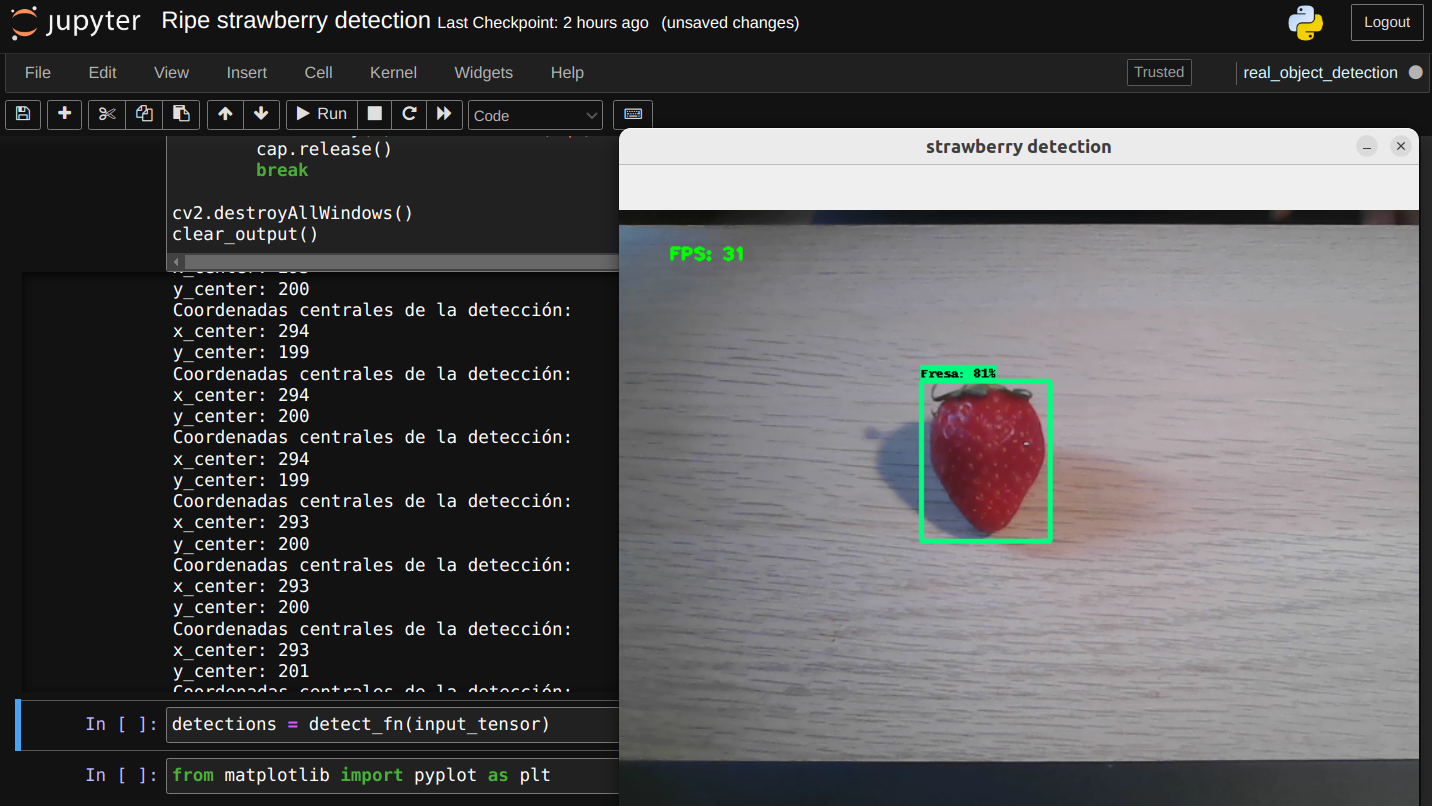
\includegraphics[width=11cm]{figs/Coordenadas centrales deteccion JN.png}
     \end{center}
     \caption{Deteccion de fresas en Jupyter Notebook}
    \label{fig:Coord_JN}
  \end{figure}

Aunque Jupyter Notebook ofrecía un entorno interactivo y muy útil no era recomendable utilizarlo como entorno de ejecución para aplicaciones estables conectadas a robots, puesto que su diseño está orientado principalmente a tareas de análisis, visualización y prototipado, donde el usuario interactúa continuamente con el entorno mediante la ejecución manual de celdas, suponiendo una limitación importante para sistemas robóticos, los cuales requieren un comportamiento determinista, autónomo y ejecutable sin supervisión constante. Una de las principales desventajas de Jupyter en este contexto es su modelo de ejecución no lineal, ya que, a diferencia de un script en Python, donde el flujo de ejecución es siempre secuencial y controlado, en un notebook es posible ejecutar fragmentos de código en cualquier orden, pudiendo provocar desincronización en las variables del programa y errores difíciles de detectar, especialmente críticos en aplicaciones donde se controla hardware, se toman decisiones en tiempo real o se actúa sobre el entorno físico. Además, a pesar de que Jupyter Notebook utiliza el lenguaje Python y puede ejecutar cualquier código compatible, su arquitectura está basada en un servidor web local que muestra la interfaz en un navegador, lo que implica que, aunque no necesita conexión a Internet, sí requiere iniciar un servidor HTTP en el sistema local, por lo que sería necesario implementar manualmente un servidor adicional dentro del propio notebook. Esto introduce una complejidad innecesaria y un entorno frágil, ya que tanto el servidor adicional como el entorno Jupyter deben mantenerse activos, y cualquier error o bloqueo en una celda puede interrumpir toda la operación.\\

Por todas estas razones, aunque Jupyter Notebook puede ser muy útil durante las fases iniciales del desarrollo para validar algoritmos de visión o procesado de datos, la implementación definitiva de un sistema conectado a un robot debe realizarse mediante scripts de Python, permitiendo un mayor control sobre el flujo de ejecución, una integración más sencilla en sistemas de control y producción, y una mayor robustez operativa, aspectos esenciales en el desarrollo de aplicaciones robóticas fiables.


\section{Detección con YOLOv3 y PyTorch}
\label{exp_seleccion_algoritmo}

Para poder comprobar las diferencias en un ejemplo práctico a la hora de detectar objetos entre PyTorch y TensorFlow, y de esta manera poder escoger una de las dos bibliotecas para el desarrollo del modelo de aprendizaje automático y aprendizaje profundo en este proyecto, se decidió crear de nuevo un entorno de Anaconda y probar a detectar objetos en imágenes utilizando Tensorflow.

\subsection{Pruebas con modelos preentrenados}
\label{sec:Pruebas_modelo_preentrenado_Pytorch}

Después de realizar la lectura \textit{You Only Look Once: Unified, Real-Time Object Detection}\cite{Redmon16}, se replicó lo que se exponía en dicho artículo con la cámara integrada del ordenador portátil, mediante un programa en Python y usando la librería Open Source Computer Vision Library (OpenCV) mediante la biblioteca Pytorch. Este programa, partiendo del \textit{feed} de la propia webcam, descomponía el vídeo en imágenes o cuadros, alimentando a la red neuronal (en este caso YOLOv3), que recibía esta detección y se procesaba con OpenCV, dibujando los recuadros o \textit{bounding box} alrededor de los objetos que se detectaban en vivo.\\

Para ello, primero se realizó la instalación de Anaconda para poder crear un ambiente de trabajo independiente y así evitar problemas entre las versiones de los paquetes necesarios para la ejecución de estas pruebas, y posteriormente se instaló OpenCV. Se clonó el repositorio \textit{deteccion-objetos-video}\footnote{\url{https://github.com/puigalex/deteccion-objetos-video}} basado en el proyecto \textit{PyTorch-YOLOv3}\footnote{\url{https://github.com/eriklindernoren/PyTorch-YOLOv3}} para correr detección de objetos sobre video y se siguieron los pasos detallados en el archivo README.
Una vez instalado todo, se probó a utilizar varios objetos y posteriormente varias frutas simultáneamente para verificar que el modelo las diferenciaba correctamente y las detectaba, tal y como se muestra en la Figura \ref{fig:Deteccion_Pytorch}.

  \begin{figure}[H]
    \begin{center}
      \subcapcentertrue
      \subfigure[Prueba deteccion de objetos con Pytorch]{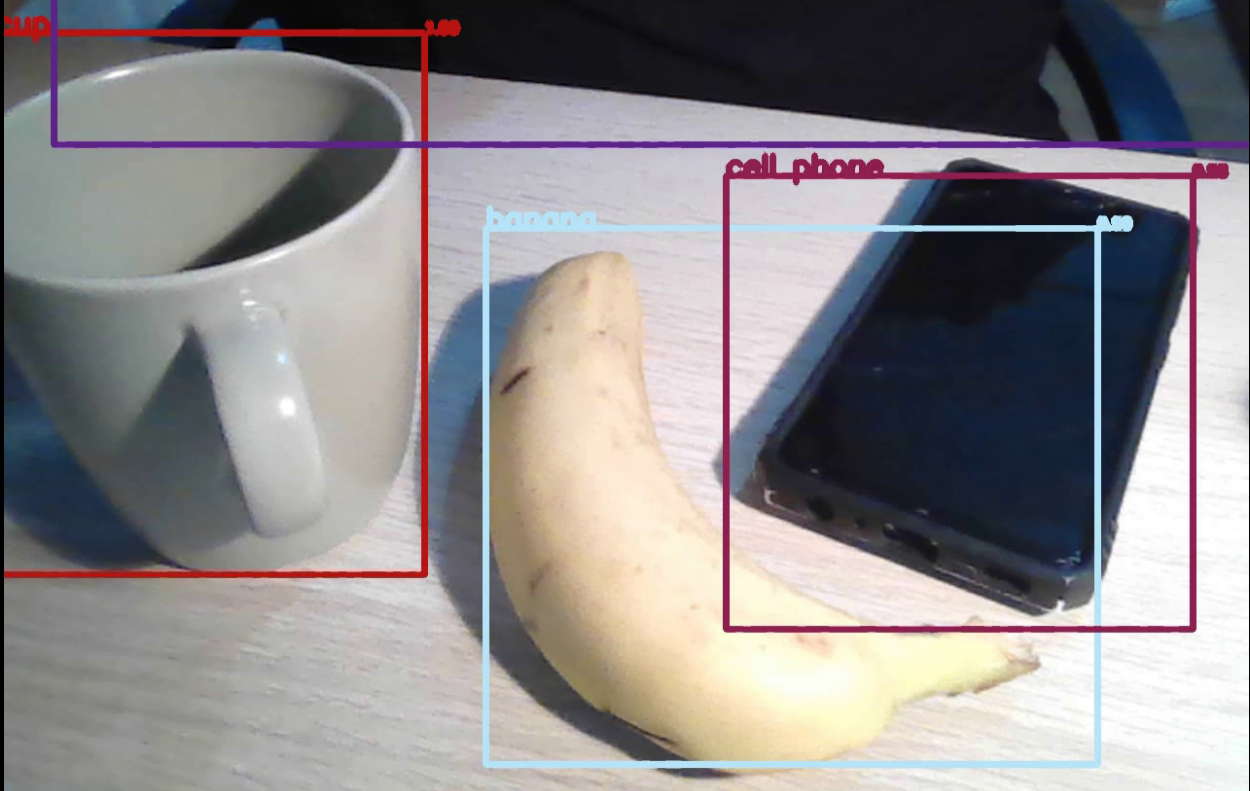
\includegraphics[width=73mm]{figs/Prueba deteccion de objetos con pytorch.png}}
      \hspace{2mm}
      \subfigure[Prueba deteccion de frutas con Pytorch]{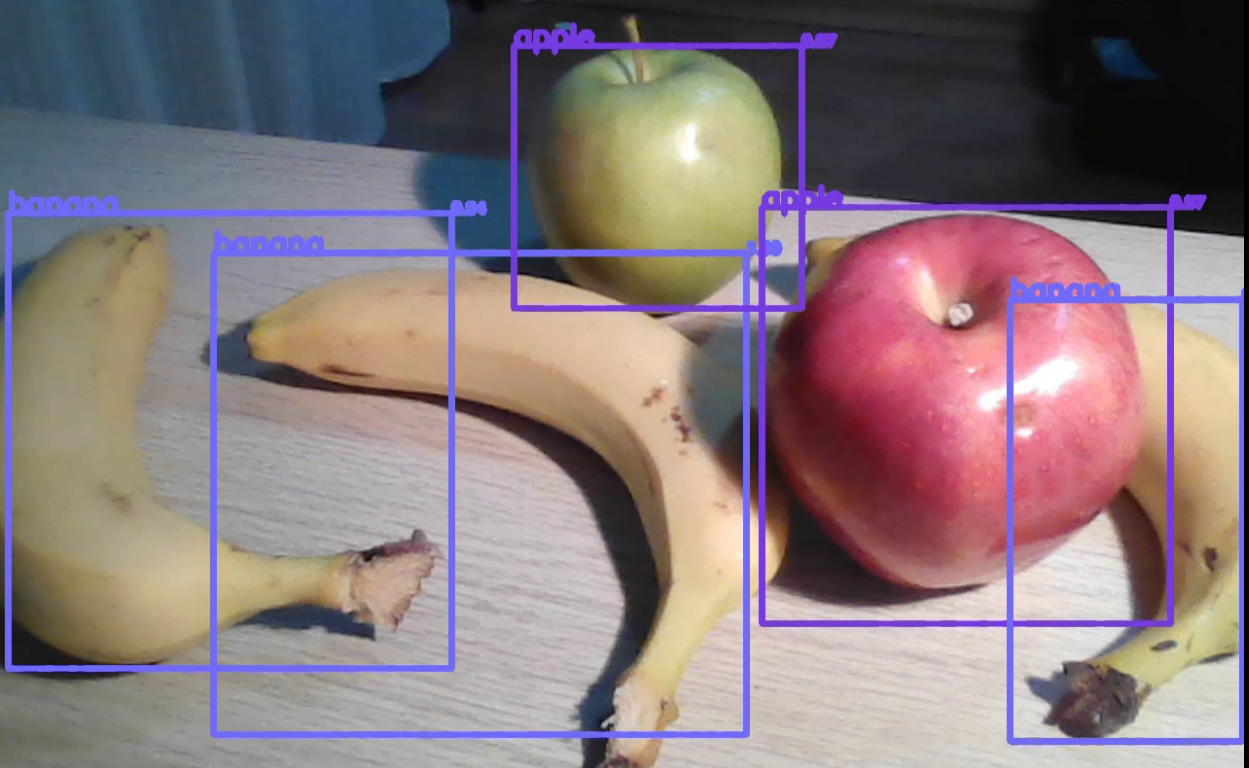
\includegraphics[width=75mm]{figs/Prueba derteccion de frutas con pytorch.png}}
    \end{center}
    \caption{Deteccion con Pytorch}
    \label{fig:Deteccion_Pytorch}
  \end{figure}
  
\subsection{Entrenamiento del modelo}
\label{sec:entrenamiento_modelo_Pytorch_Python}


Debido a que, tras la detección de las posiciones de las fresas mediante el programa de Jupyter Notebook, no se puede trabajar directamente con ellas y enviarlas al robot, ya que Jupyter Notebook está basado en web, por lo que haría falta un servidor web intermediario para esto, tal y como se explicó en el apartado anterior, se intentó llevar a cabo la elaboración del programa de detección en Python, para que de este modo se pudieran enviar al brazo robótico directamente las coordenadas, al estar trabajando en local y tener todo el código unificado. Además, se sustituyó TensorFlow por PyTorch como biblioteca de desarrollo del modelo de visión, basándose en que PyTorch ofrece una sintaxis más intuitiva y cercana a la programación en Python puro, lo que facilita su integración con scripts que deben ejecutarse en tiempo real junto con otros módulos, como los encargados de la comunicación con el robot, además de que PyTorch presenta una curva de aprendizaje más suave para depuración y prototipado rápido, y proporciona una mayor facilidad a la hora de exportar modelos, optimizarlos o ajustarlos dinámicamente durante la ejecución, resultando ser más adecuado para un sistema unificado, local y modular que debe ejecutarse de forma autónoma, sin depender de interfaces gráficas ni entornos web como Jupyter.\\

Para ello se tomó como referencia y ayuda los repositorios \textit{Real Time Emotion Detection for Low Cost Robot in ROS}\footnote{\url{https://github.com/jamarma/emotion_detection_ros}} y \textit{Detección de objetos en vídeo}\footnote{\url{https://github.com/puigalex/deteccion-objetos-video}} y se creó un entorno nuevo en Anaconda llamado \textit{deteccionobj}.\\

Durante el entrenamiento del modelo, surgieron varios códigos de error relacionados con el etiquetado de las imágenes utilizadas para esto, por lo que se decidió etiquetarlas de nuevo mediante el programa labelImg (Figura \ref{fig:labelImg_Fresas}), tal y como se había hecho anteriormente con TensorFlow.

 \begin{figure}[H]
     \centering
     \begin{center}
       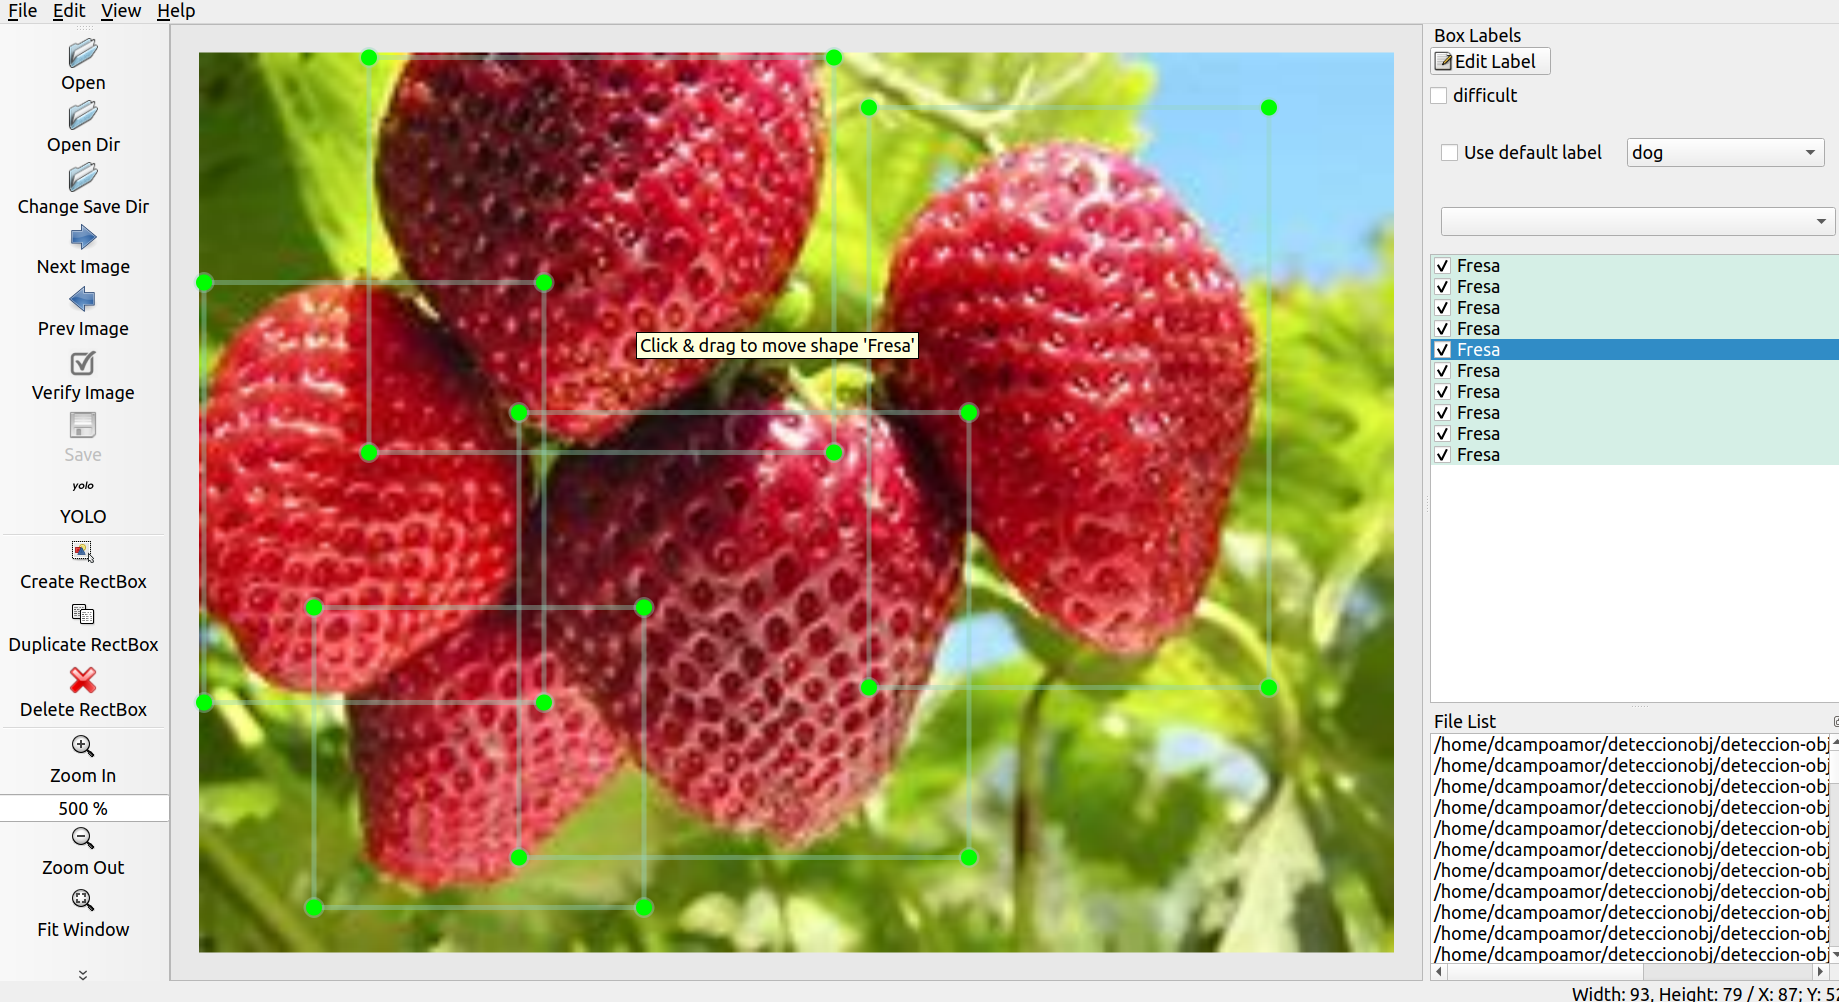
\includegraphics[width=11cm]{figs/labelImg Fresa.png}
     \end{center}
     \caption{Etiquetado de las imágenes con labelImg}
    \label{fig:labelImg_Fresas}
  \end{figure}

Finalizado el proceso de etiquetado de 432 imágenes, se almacenaron en la carpeta \textit{labels} los archivos que incluían tanto el número de clase, identificado con el valor 0, correspondiente a la única clase considerada, "Fresa",  como las coordenadas que delimitaban la ubicación del objeto dentro de cada imagen. Con esta información organizada, se procedió al entrenamiento del modelo utilizando la arquitectura Darknet-53, implementada en el framework Darknet, más concretamente se empleó el archivo darknet53.conv.74, correspondiente a las primeras 74 capas de la red preentrenadas con pesos convolucionales, lo cual permitió una inicialización eficiente y evitó entrenar el modelo YOLO desde cero.\\

Para el entrenamiento, se configuró el parámetro batch\_size con un valor de 2, debido a las limitaciones de capacidad de la tarjeta gráfica empleada, lo que implicó que las imágenes se procesaran de dos en dos por iteración. Además, al finalizar cada época del entrenamiento, entendida como el momento en que la red ha procesado y actualizado todos los ejemplos del conjunto de entrenamiento, se generó un checkpoint con los pesos actuales del modelo, almacenado en la carpeta correspondiente, dando lugar a un total de 100 checkpoints al concluir el proceso dado que el entrenamiento fue configurado por defecto para ejecutarse durante 100 épocas.

\subsection{Calibrado de la cámara}
\label{sec:Calibrado_camara}

Con el fin de optimizar la detección de objetos mediante YOLOv3 y PyTorch, se procedió a la calibración de la cámara web de Logitech C270, determinando sus parámetros intrínsecos y la transformación de su sistema de coordenadas respecto al entorno. Para ello, se utilizaron 20 imágenes de un patrón de tablero de ajedrez en diferentes posiciones, tomadas con la cámara a calibrar, mediante las cuales, y a través del uso del programa \textit{PiCamCalibrator.py}\footnote{\url{https://github.com/RoboticsURJC/tfg-dcampoamor/blob/main/src/piCamCalibrator/PiCamCalibration.py}}, se obtenían estos valores de la matriz K, como muestra la Figura \ref{fig:calibracion_camara}. 

 \begin{figure}[H]
    \begin{center}
      \subcapcentertrue
      \subfigure[Chess board]{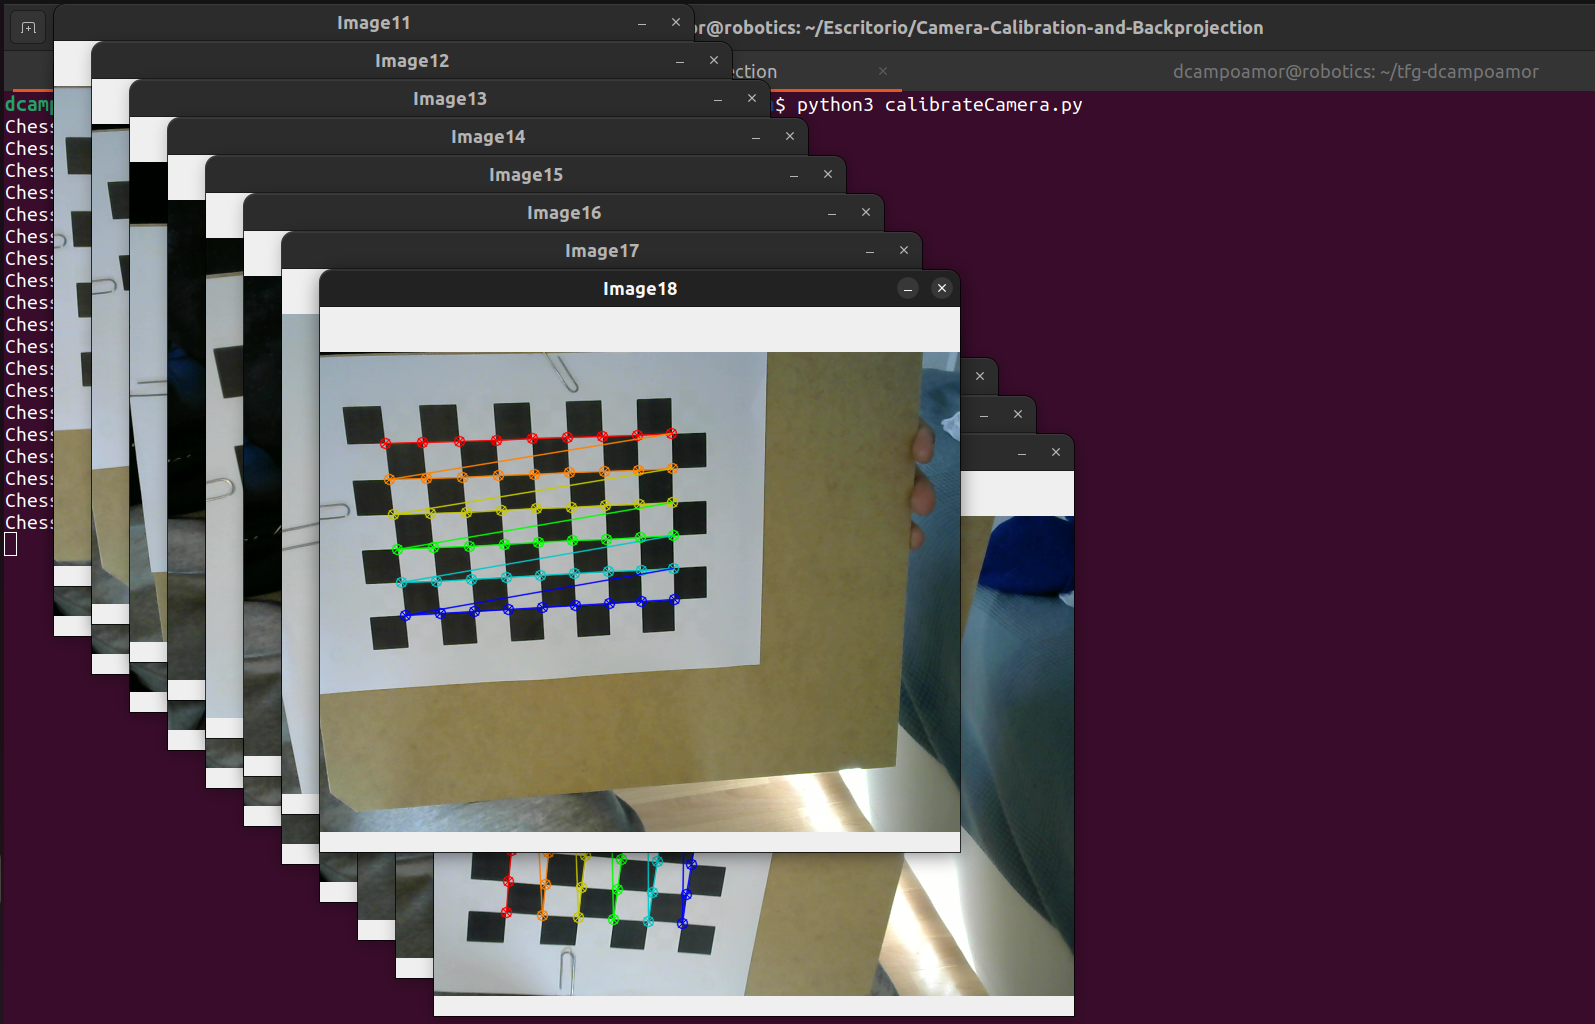
\includegraphics[height=40mm, width=73mm]{figs/calibrateCamera.png}}
      \hspace{2mm}
      \subfigure[Parámetros intrínsecos de la cámara]{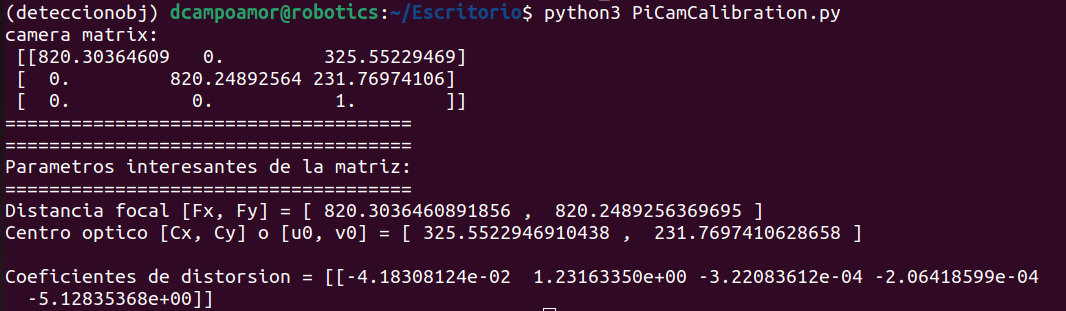
\includegraphics[height=40mm, width=75mm]{figs/matriz K camara.png}}
    \end{center}
    \caption{Calibración de la cámara C270 de Logitech}
    \label{fig:calibracion_camara}
  \end{figure}

Para corroborar si esta primera calibración de la cámara C270 de Logitech había sido buena, se llevaron a cabo diez calibraciones más para comprobar los resultados entre sí con diferentes imágenes tomadas con el mismo \textit{chess board}, siendo los valores tomados para la programación, la media aritmética entre todas las mediciones.

Junto con las matrices de Rotación R y la matriz de Traslación T de la cámara, se realizó el cálculo de la transformación del sistema de coordenadas que viene definido por la multiplicación de las tres matrices, para lo cuál, se instaló la cámara en un trípode, cuya altura al plano mesa conocíamos, y con una inclinación de la cámara medida mediante la aplicación de ERGONAUTAS RULER - Medición de ángulos en fotografías y vídeos\footnote{\url{https://www.ergonautas.upv.es/herramientas/ruler/ruler.php}} de la Universidad Politécnica de Valencia, como se aprecia en la Figura \ref{fig:medicion_angulo_ERGONAUTAS}.

 \begin{figure}[H]
     \centering
     \begin{center}
       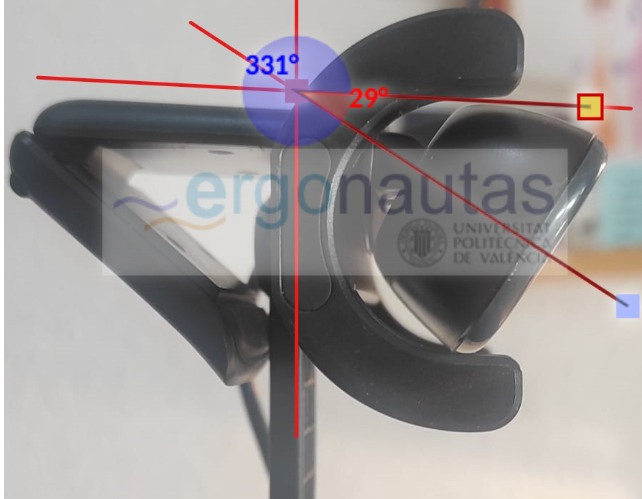
\includegraphics[width=80mm]{figs/ERGONAUTAS Medicion angulo.png}
     \end{center}
     \caption{Medición del ángulo de rotación de la cámara mediante la aplicación de ERGONAUTAS RULER}
    \label{fig:medicion_angulo_ERGONAUTAS}
  \end{figure}


\subsection{Pruebas detección de fresas en tiempo real}
\label{sec:Pruebas_Fresas_Pytorch}

Una vez con el modelo entrenado, se realizaron las primeras pruebas utilizando Python de detección de fresas en tiempo real, para las que se utilizó la cámara integrada del ordenador portátil e imágenes de fresas en el móvil mediante el programa \textit{deteccion\_video.py}\footnote{\url{https://github.com/RoboticsURJC/tfg-dcampoamor/blob/main/src/deteccion-objetos-video/deteccion_video.py}}, tal y como se muestra en la Figura \ref{fig:primerasdetecciones_Python}, y a partir de las cuales se modificaron tanto el grosor del nombre de la clase a detectar como el threshold de la detección mostrado en la ventana emergenteen con OpenCV, ajustándolde tal manera quemo argumento que pudieran ser más legibles en el programa.

  \begin{figure}[H]
     \centering
     \begin{center}
       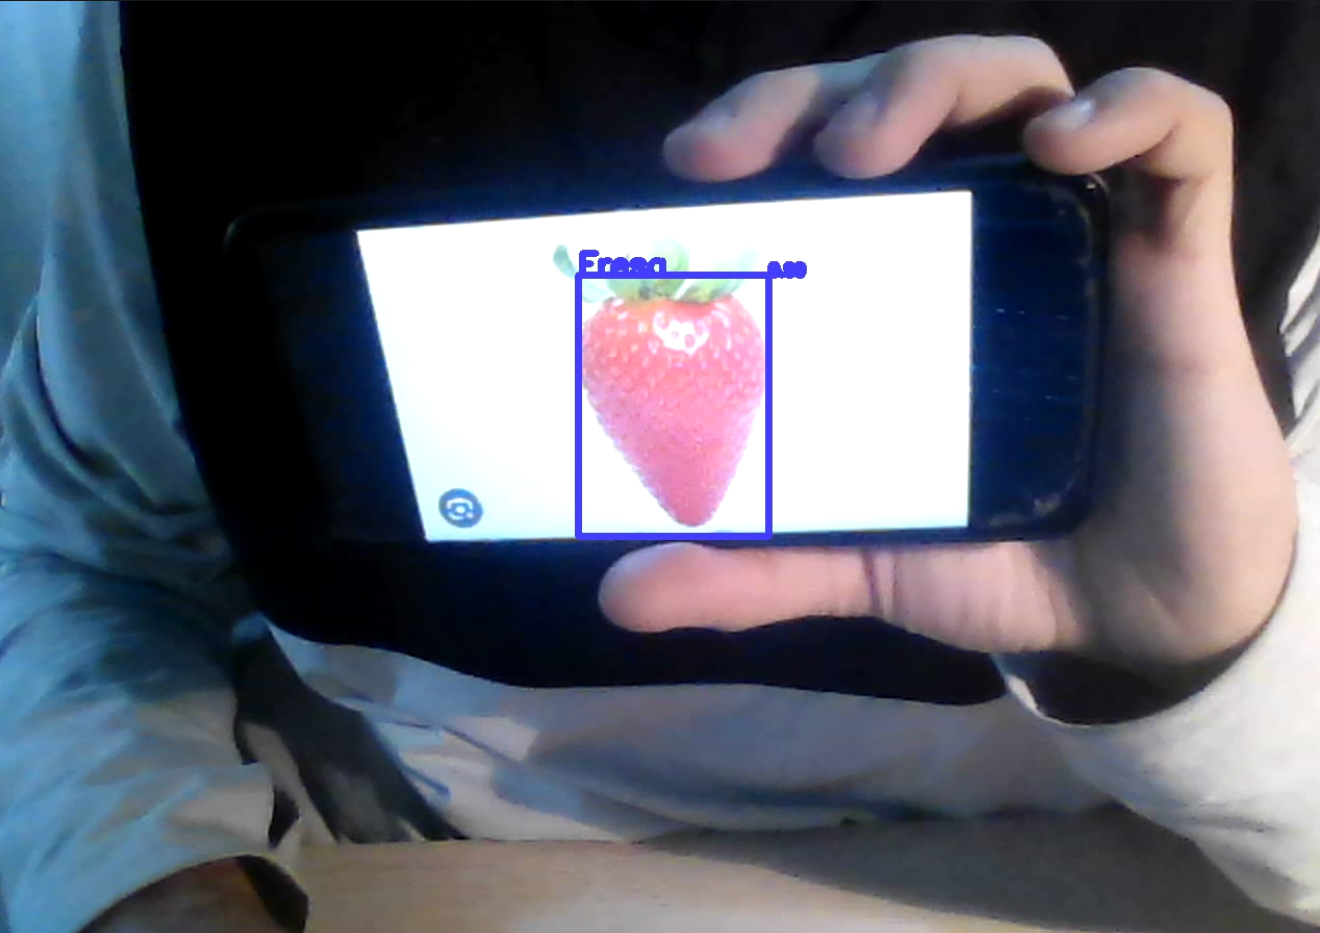
\includegraphics[width=80mm]{figs/deteccion_video fresa en foto.png}
     \end{center}
     \caption{Primeras pruebas de detección con PyTorch y Python}
    \label{fig:primerasdetecciones_Python}
  \end{figure}

Sobre esta primera versión se fue modificando el código para poder añadir más funcionalidades al sistema, como la incorporación de un fragmento diseñado para almacenar dinámicamente las coordenadas centrales de los recuadros de las fresas detectadas por el modelo en una lista, y, dado que la versión inicial del script no consideraba la posible redundancia en la detección, es decir, la identificación múltiple de un mismo objeto debido a ligeras variaciones en la posición, también se incorporó un criterio de tolerancia espacial, que permitiera verificar si una nueva detección se encontraba a una distancia euclidiana inferior al umbral respecto a alguna de las posiciones ya registradas, y en tal caso, la nueva posición no se añadiría a la lista, evitando así duplicidades en las detecciones.\\

Paralelamente a esto, con el fin de verificar los cálculos de las transformaciones entre sistemas de coordenadas, y poder obtener las distancias a las que se encontraban las detecciones de la cámara, se desarrolló el programa \textit{pos\_centroide.py}\footnote{\url{https://github.com/RoboticsURJC/tfg-dcampoamor/blob/main/src/camera/pos_centroide.py}} en lenguaje Python. Este script utilizaba la biblioteca OpenCV para realizar la detección de un objeto a partir de un filtro por color, calculando su centroide y devolviendo el resultado en pixeles. A partir de estas coordenadas en píxeles, era posible obtener las coordenadas en el sistema óptico de la cámara y finalmente a partir de estas coordenadas en 2D, proyectar el punto en el espacio tridimensional (3D) utilizando los parámetros intrínsecos y extrínsecos de la cámara, permitiendo así obtener las coordenadas espaciales X,Y,Z que se mostraban en la terminal como salida del programa. \\

Se utilizó un cuadrado de un post-it subrayado con color amarillo fosforescente sobre una cartulina blanca para poder minimizar el error cometido por el programa al aplicar el filtro de color y poder calcular así de mejor manera las distancias y coordenadas del centroide de ese cuadrado. Para estas pruebas, se supuso un sistema de referencia cartesiano, donde el eje Z el perpendicular al plano de la mesa, es decir, la altura a la que se encontraba instalada la cámara a la hora de realizar las pruebas para poder seguir el principio de la hipótesis suelo, mientras que en un principio, se supuso el eje X como el eje longitudinal de la mesa y el eje Y el transversal de la misma. No obstante, se realizaron más mediciones desplazando el post-it en distintas direcciones para poder validar estas suposiciones sobre la configuración del sistema de coordenadas y ajustar su orientación a fin de asegurar la correspondencia entre los resultados estimados por el sistema y las coordenadas reales del entorno (Figura \ref{fig:primera_estimacion_postit}).

  \begin{figure}[H]
     \centering
     \begin{center}
       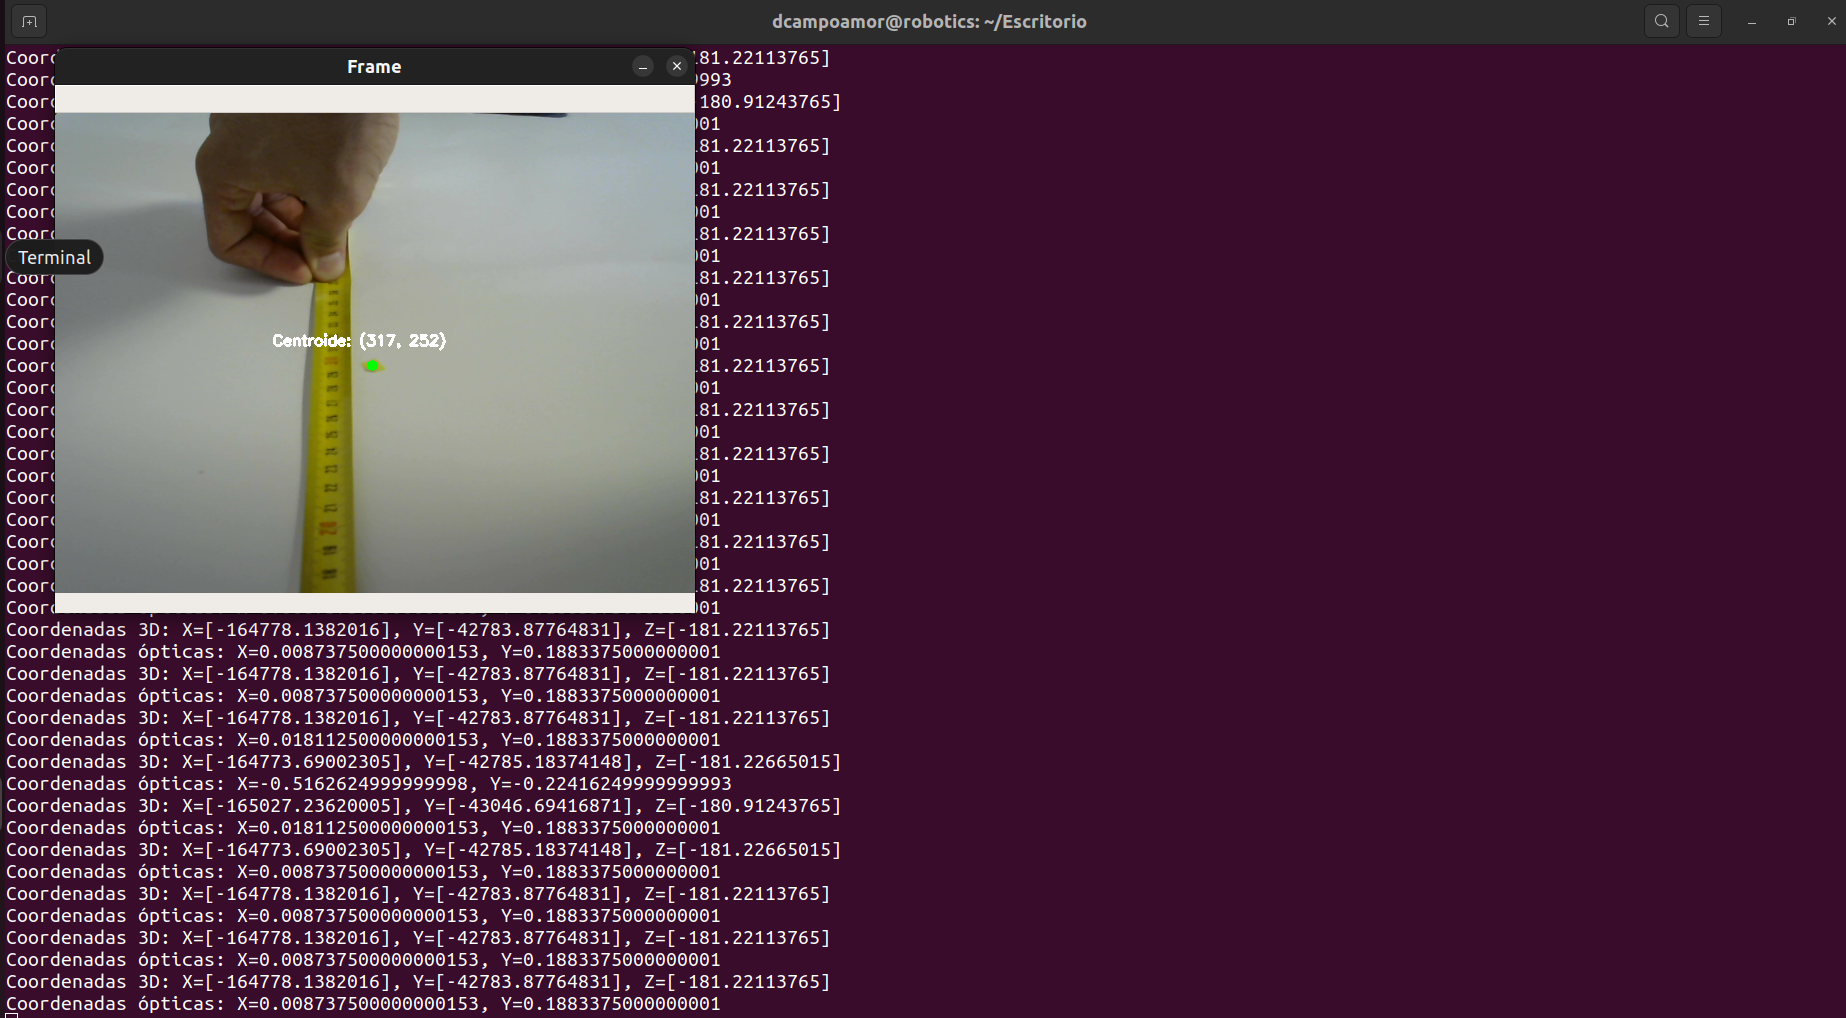
\includegraphics[width=115mm]{figs/Punto inicial 30cm.png}
     \end{center}
     \caption{Primeras pruebas de la estimación de las coordenadas y la distancia de la detección a la cámara}
    \label{fig:primera_estimacion_postit}
  \end{figure}

De los resultados de estas mediciones, recogidos en el Cuadro \ref{tab:primerosresultados_postit}, se observó que existía algún tipo de error en el proceso de cálculo, posiblemente en las transformaciones aplicadas o a la omisión de algún factor relevante, ya fuera geométrico o de calibración, ya que se manifestaba en la falta de concordancia entre las coordenadas espaciales reales y las estimadas por el sistema, a pesar de que se pudo comprobar que los valores obtenidos presentan una coherencia relativa, al variar conforme estos desplazamientos.

  \begin{table}[H]
     \centering
     \begin{center}
       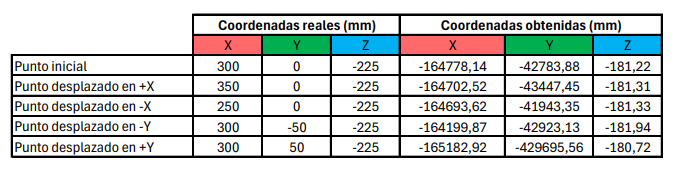
\includegraphics[width=140mm]{figs/Primer resultados postit.png}
     \end{center}
     \caption{Comparacion entre coordenadas reales y obtenidas (en mm)}
    \label{tab:primera_estimacion_postit}
  \end{table}

Ante estas discrepancias, se procedió a consultar bibliografía útil para este ámbito, concretamente el documento \textit{Real World Coordinate from Image Coordinate Using Single Calibrated Camera}\cite{Joko13}, donde se analizaba la geometría del modelo de cámara basado en el modelo estenopeico o modelo pinhole (Figura \ref{fig:geometria_modelopinhole}), cuya figura se empleó como referencia para verificar la correcta definición y orientación de los ejes del sistema de coordenadas. Esta revisión permitió contrastar las hipótesis iniciales relativas a los ejes sobre los que se aplican las rotaciones de la cámara, así como los ejes en los que se realizaron las mediciones experimentales, con el objetivo de detectar posibles inconsistencias en la configuración del sistema de referencia adoptado.

  \begin{figure}[H]
     \centering
     \begin{center}
       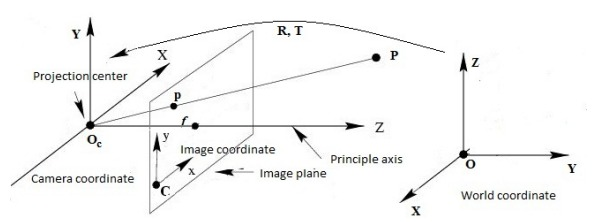
\includegraphics[width=135mm]{figs/Geometría del modelo de cámara basado en el modelo de cámara estenopeica.jpeg}
     \end{center}
     \caption{Geometría basada en el modelo de cámara estenopeica}
    \label{fig:geometria_modelopinhole}
  \end{figure}

Dado que los resultados experimentales mostraban una desviación considerable respecto a las distancias reales y no se lograba establecer una relación clara y precisa, se optó por adoptar un enfoque alternativo basado en un script preexistente denominado \textit{pinhole.py}\footnote{\url{https://github.com/RoboticsURJC/tfg-dcampoamor/blob/main/src/camera/cameraPibot/pinhole.py}}, que implementaba el modelo de cámara estenopeica para estimar coordenadas espaciales a partir de coordenadas de un imagen o vídeo. Se ajustaron diversos parámetros globales fundamentales, tales como el ancho y alto de la imagen, la distancia focal y la posición del centro óptico de la cámara, datos obtenidos anteriormente en la calibración de la cámara, así como variables asociadas a la rotación de la misma, como el ángulo de inclinación de la cámara, y a la traslación o altura de la cámara respecto a la superficie de trabajo, con el fin de calcular adecuadamente las matrices de rotación y traslación necesarias para la proyección de puntos desde el espacio imagen al espacio real. Además, se adaptó el rango de detección cromática para que, al ejecutar el script, pudiera detectarse el color amarillo característico del post-it sobre la cartulina blanca dispuesta sobre la mesa, facilitando así la identificación automática del objeto en las pruebas, tal y como se había hecho con scripts anteriores.\\

Se estableció como origen del sistema de coordenadas del mundo la proyección vertical del centro óptico de la cámara sobre la superficie de la mesa, y se llevaron a cabo distintas pruebas experimentales, modificando tanto el signo del ángulo de rotación como el signo de la distancia de la cámara a la mesa, cuya medida era de 22º para estos experimentos, con el objetivo de determinar la orientación correcta de los ejes espaciales definidos en el script y verificar si los resultados estimados se correspondían con las coordenadas reales. Para la recogida de datos, se empleó una regla graduada colocada sobre la superficie de la mesa, y se fue desplazando de manera progresiva el post-it en distintas direcciones para poder validar las suposiciones sobre la configuración del sistema de coordenadas (Figura \ref{fig:prueba_ejes_camara}).

 \begin{figure}[H]
    \begin{center}
      \subcapcentertrue
      \subfigure[Medidas en el eje longitudinal de la mesa]{\includegraphics[width=71mm]{figs/Pruebas pinhole único eje.png}}
      \hspace{2mm}
      \subfigure[Medidas en el eje transversal de la mesa]{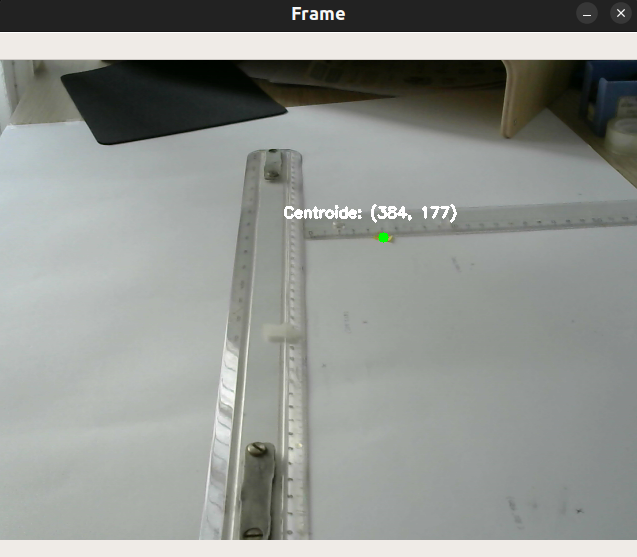
\includegraphics[width=72mm]{figs/Pruebas pinhole ambos ejes.png}}
    \end{center}
    \caption{Pruebas para determinar la configuración del sistema de coordenadas de la cámara}
    \label{fig:prueba_ejes_camara}
  \end{figure}
  
A partir de los resultados obtenidos en estas pruebas, recogidos en los Cuadros \ref{tab:pinhole_Zpos} y \ref{tab:pinhole_Zneg}, se pudo comprobar que, para que las estimaciones del sistema fueran coherentes con las distancias reales, era necesario introducir la altura de la cámara respecto al plano suelo, en este caso, la mesa, como un valor negativo, mientras que el ángulo de rotación de la cámara debía establecerse en valor positivo. Esta configuración permitía que, al alejar el post-it amarillo del origen, la distancia estimada aumentara progresivamente, tal y como era esperable. 
  
  \begin{table}[H]
    \centering
    \begin{center}
      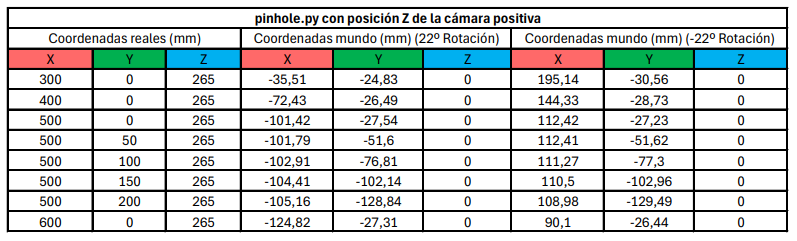
\includegraphics[width=150mm]{figs/pinhole con Z positiva.png}
    \end{center}
    \caption{Resultados del programa pinhole.py con valores de Z positivos}
    \label{tab:pinhole_Zpos}
  \end{table}
  
  
  \begin{table}[H]
   \centering
   \begin{center}
     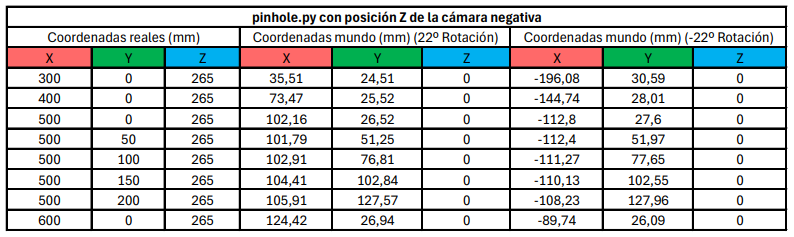
\includegraphics[width=150mm]{figs/pinhole con Z negativa.png}
   \end{center}
   \caption{Resultados del programa pinhole.py con valores de Z negativos}
   \label{tab:pinhole_Zneg}
  \end{table}

No obstante, a pesar de haber definido un sistema de coordenadas inicial, los resultados continuaban sin ajustarse adecuadamente a las distancias reales, por ello, se decidió revisar en mayor detalle la lógica del script \textit{pinhole.py}, prestando especial atención a los comentarios incluidos en el código, en los que se indicaba que los ángulos utilizados para calcular la matriz de rotación se definían bajo la suposición de que la cámara, en orientación vertical, había sido sometida a una rotación previa de 90 grados sobre el eje Y. A partir de esta observación, se procedió a representar y analizar el sistema de coordenadas original de la cámara antes de aplicar dicha transformación, con el objetivo de comprender mejor la correspondencia entre los ejes del sistema imagen y del sistema mundo, y así ajustar de forma más precisa las transformaciones necesarias (Figura \ref{fig:esquema_rot_camara}). 

  \begin{figure}[H]
     \centering
     \begin{center}
       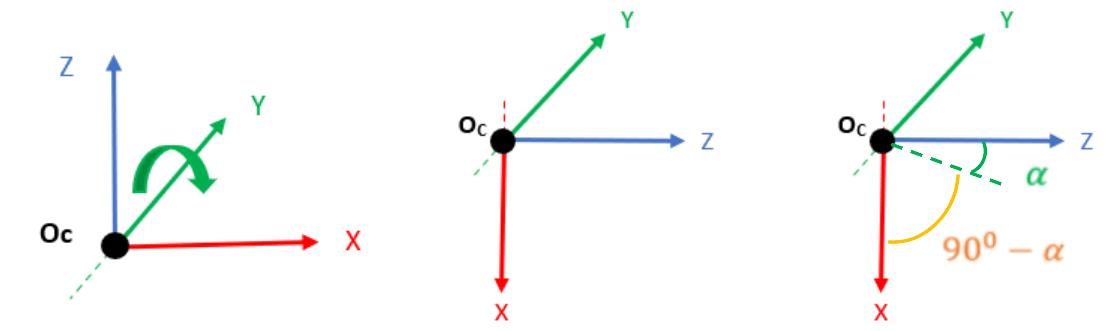
\includegraphics[width=100mm]{figs/Esquema rotación cámara.png}
     \end{center}
     \caption{Esquema de la rotación de la cámara}
    \label{fig:esquema_rot_camara}
  \end{figure}

Se consideró entonces una rotación sobre el eje vertical de la cámara, y se utilizó como ángulo de entrada para el código, el valor resultante de restar los 90° de la rotación inicial asumida en el script menos el ángulo previamente utilizado (definido como el ángulo entre la horizontal y la dirección de la lente). El valor resultante en esta ocasión fue de aproximadamente 65°, con el cual se volvió a ejecutar el script, a fin de evaluar si esta nueva configuración ofrecía una mayor coherencia entre las coordenadas estimadas y las medidas reales, repitiendo las mismas pruebas definidas anteriormente y obteniendo los resultados del Cuadro \ref{tab:pinhole_rot_camara}.

   \begin{table}[H]
   \centering
   \begin{center}
     \includegraphics[width=95mm]{figs/Resultados mediciones pinhole 65º Rotacion.png}
   \end{center}
   \caption{Resultados del programa pinhole.py con el valor ajustado de rotación de la cámara}
   \label{tab:pinhole_rot_camara}
  \end{table}
  
Una vez verificada y establecida la forma correcta de introducir los parámetros relativos al ángulo de inclinación y a la altura de la cámara respecto al plano suelo, ya que pudieron considerarse satisfactorios debido a su similitud con las mediciones reales, se procedió a incorporar en el propio script el cálculo de la distancia a partir de las coordenadas tridimensionales (X,Y,Z) del punto detectado, desarrollando para ello la función \textit{calcular\_distancia\_3d}, que permitía estimar la distancia euclídea desde el origen del sistema hasta el punto proyectado (Figura \ref{fig:dist_camara}). 

   \begin{figure}[H]
    \begin{center}
      \subcapcentertrue
      \subfigure[Detección y cálculo de las coordenadas y la distancia a la detección]{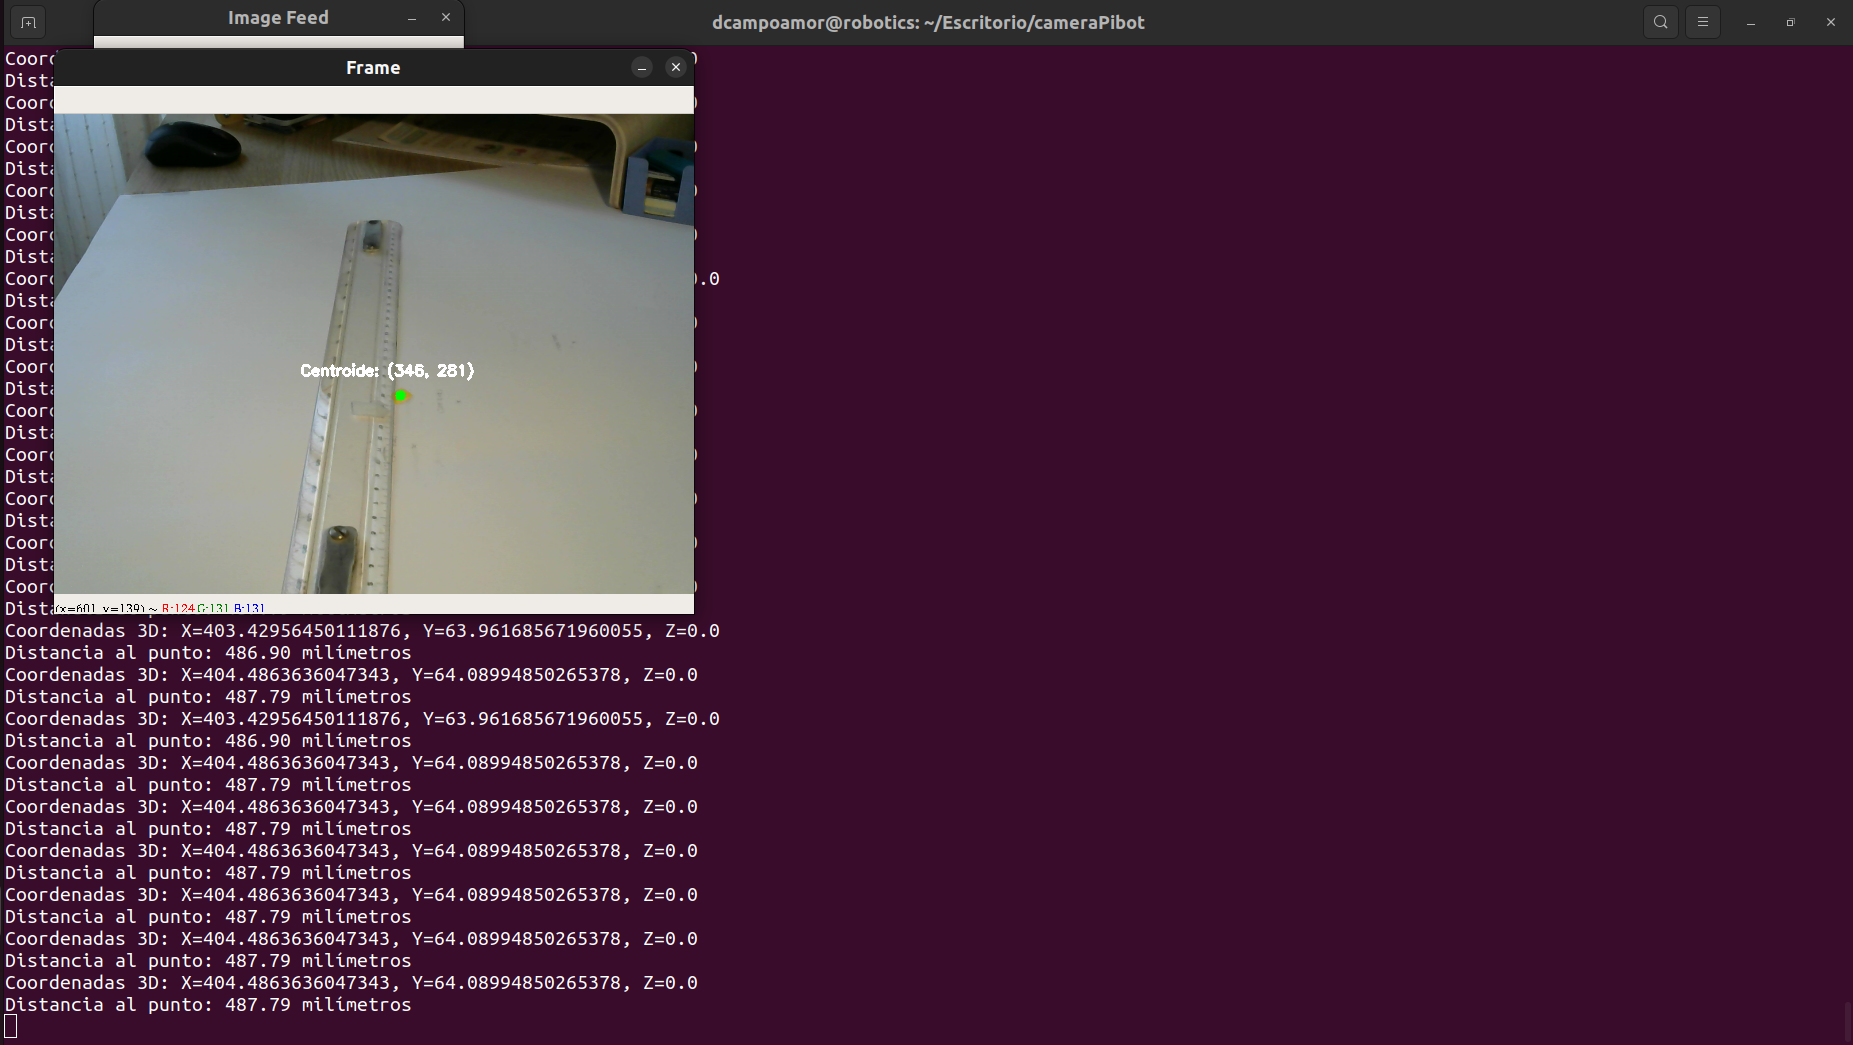
\includegraphics[height=50mm, width=70mm]{figs/Deteccion puntos y distancia EJE X.png}}
      \hspace{2mm}
      \subfigure[Comprobación de la medición de la distancia de la cámara a la detección]{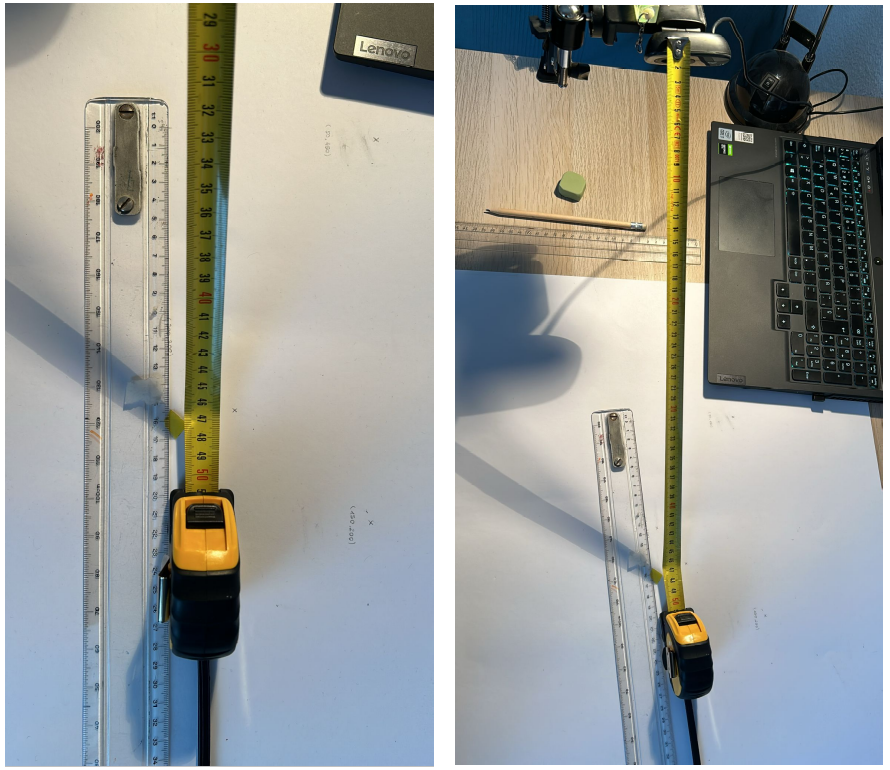
\includegraphics[height=50mm, width=75mm]{figs/Distancia al punto.png}}
    \end{center}
    \caption{Cálculo de la distancia de la cámara a la detección}
    \label{fig:dist_camara}
  \end{figure}

Dado que el programa \textit{pinhole.py} permitía inicialmente la detección de un único punto amarillo dentro de la escena, en línea con el enfoque de las pruebas preliminares, centradas en validar el funcionamiento del sistema y la precisión del cálculo de la posición y la distancia del objeto respecto a la cámara, surgía una limitación evidente al poder darse la posibilidad de trabajar con múltiples detecciones. Para permitir la detección simultánea, se modificó este programa, generando uno nuevo denominado \textit{pinhole\_deteccionmultiple.py}\footnote{\url{https://github.com/RoboticsURJC/tfg-dcampoamor/blob/main/src/camera/cameraPibot/pinhole_deteccionmultiple.py}}, y se procedió en primer lugar a ajustar los filtros de color del sistema, ya que en el entorno de pruebas existían varios elementos de madera cuyas tonalidades se confundían con el amarillo claro bajo determinadas condiciones de iluminación, generando falsas detecciones, por lo que, para mitigar este problema, se optó por reemplazar el color amarillo por el verde, lo que implicó también pintar los fragmentos de post-it utilizados en las pruebas con este nuevo color. Una vez realizada esta modificación, se implementaron mejoras adicionales, como la numeración de los objetos detectados para permitir identificar de forma unívoca cada detección dentro del mismo escenario, lo cual resultaba esencial para poder asociar correctamente las coordenadas espaciales y las distancias estimadas con cada objeto individual, ampliando la capacidad del sistema para trabajar en escenarios más complejos con múltiples puntos de interés (Figura \ref{fig:deteccion_multiple_ptos}).

   \begin{figure}[H]
   \centering
   \begin{center}
     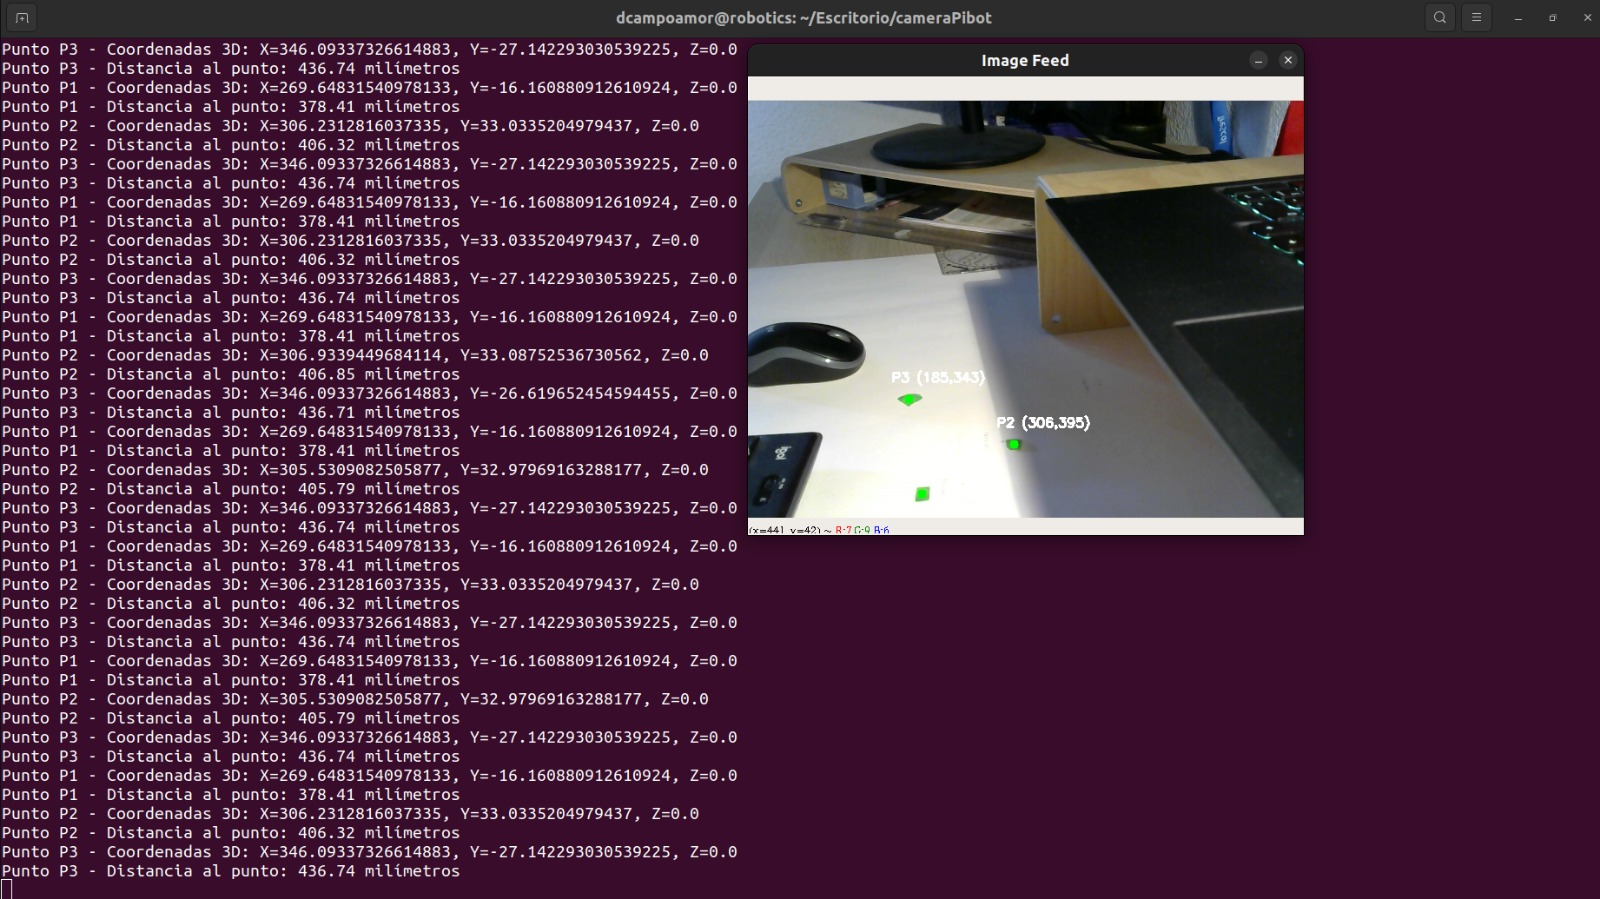
\includegraphics[width=110mm]{figs/Deteccionmultiple ejemplo.png}
   \end{center}
   \caption{Detección múltiple simultánea de post-it}
   \label{fig:deteccion_multiple_ptos}
  \end{figure}
  
Una vez resueltas las limitaciones iniciales del programa \textit{pinhole.py} en cuanto a la detección de múltiples objetos, y tras haber conseguido proyectar correctamente los centroides de los objetos detectados junto con el cálculo de sus coordenadas espaciales y distancias respectivas, se avanzó en la representación visual de estos resultados modificando el script \textit{pinhole\_deteccionmultiple.py} para que, además de realizar la detección y proyección de múltiples detecciones de manera simultánea, se capturaran y representaran estos datos en una ventana adicional mediante OpenGL. Para ello, se reutilizaron y adaptaron las funcionalidades de navegación y visualización incluidas en el script \textit{scene\_navigation.py}\footnote{\url{https://github.com/RoboticsURJC/tfg-dcampoamor/blob/main/src/camera/openglhw/scene_navegation.py}}, que permitía representar escenas 3D de forma interactiva mediante el uso de \textit{multithreading}, una técnica de programación que permite ejecutar múltiples tareas concurrentemente dentro de un mismo proceso. Tras varias pruebas y ajustes en la integración de ambos scripts, se consiguió que los puntos detectados por la cámara se representaran correctamente en una ventana paralela con fondo negro utilizando OpenGL, mostrándose cada punto como una marca roja en el espacio tridimensional, pero para mejorar la visibilidad y el contraste de estos puntos, se modificó tanto el tamaño de los puntos comoo la selección del color para que fuera más perceptible frente al fondo y se añadieron líneas entre los puntos detectados, tal y como se muestra en la Figura \ref{fig:dist_camara}. Esta representación permitió verificar visualmente la coherencia de las coordenadas 3D calculadas a partir de la cámara, facilitando así la validación y comprensión de los resultados espaciales obtenidos durante las pruebas anteriores.

    \begin{figure}[H]
      \begin{center}
        \subcapcentertrue
        \subfigure{\includegraphics[height=43mm, width=75mm]{figs/pinhole_openGL ventana cuadrado.png}}
        \hspace{1mm}
        \subfigure{\includegraphics[width=75mm]{figs/pinhole_openGL triangulo.png}}
      \end{center}
      \caption{Representación de las detecciones con OpenGL}
      \label{fig:dist_camara}
    \end{figure}

Una vez validado el funcionamiento del sistema con fragmentos de post-it pintados, y comprobada la capacidad del programa para detectar múltiples puntos, calcular sus coordenadas espaciales, se consideró que el sistema estaba preparado para abordar el siguiente paso del proyecto: sustituir los objetos de prueba por el objeto real de estudio, las fresas, por lo que se inició una nueva fase centrada en la detección, localización y estimación de la distancia a estas detecciones de fresas en condiciones más próximas a las del entorno operativo final, recogida en el programa \textit{xmlrpc\_deteccionfresas.py}\footnote{\url{https://github.com/RoboticsURJC/tfg-dcampoamor/blob/main/src/deteccion-objetos-video/xmlrpc_deteccionfresas.py}}. Para ello, fue necesario modificar algunos parámetros del sistema y sustituir el método de detección basado en filtros de color, empleado durante las pruebas iniciales, por el modelo de detección entrenado específicamente para identificar fresas, que ya se encontraba integrado en el script \textit{deteccion\_video.py}, por lo que se reutilizó dicha lógica adaptándola al flujo de trabajo del sistema basado en pinhole.py, obteniendo los resultados de la Figura \ref{fig:union_scripts_fresas}.

  \begin{figure}[H]
    \centering
    \begin{center}
      \includegraphics[width=110mm]{figs/Pruebas deteccion fresas y obtencion coordenadas varios codigos.png}
    \end{center}
    \caption{Detección de fresas e integración con el sistema de cálculo de coordenadas y distancias}
    \label{fig:union_scripts_fresas}
  \end{figure}

Sin embargo, la integración del modelo de detección de fresas no fue un proceso directo, ya que el cambio de un método de detección basado en filtrado de color a uno basado en inteligencia artificial implicó importantes ajustes, ya que las características de la detección variaban considerablemente. Debido a esta modificación, fue necesario repetir las pruebas de estimación de coordenadas y distancias, con el fin de verificar nuevamente la orientación del sistema de coordenadas y asegurar que las nuevas detecciones proporcionadas por el modelo se proyectaran correctamente en el espacio tridimensional. Estas pruebas permitieron recalibrar el sistema en función del nuevo flujo de trabajo (ver Cuadros \ref{tab:resultados_145mm_59grados}, \ref{tab:resultados_125mm_59grados} \ref{tab:resultados_225mm_69grados} y \ref{tab:resultados_180mm_58grados}).

   \begin{table}[H]
     \centering
     \begin{center}
       \includegraphics[width=155mm]{figs/Resultados 145 mm 59 grados.png}
     \end{center}
     \caption{Resultados del programa xmlrpc\_deteccionfresas.py con la cámara situada a 145 mm de la mesa y la cámara rotada 59 grados}
     \label{tab:resultados_145mm_59grados}
  \end{table}
  
  \begin{table}[H]
     \centering
     \begin{center}
       \includegraphics[width=155mm]{figs/Resultados 125 mm 59 grados.png}
     \end{center}
     \caption{Resultados del programa xmlrpc\_deteccionfresas.py con la cámara situada a 125 mm de la mesa y la cámara rotada 59 grados}
     \label{tab:resultados_125mm_59grados}
  \end{table}

  \begin{table}[H]
     \centering
     \begin{center}
       \includegraphics[width=155mm]{figs/Resultados 225 mm 69 grados.png}
     \end{center}
     \caption{Resultados del programa xmlrpc\_deteccionfresas.py con la cámara situada a 225 mm de la mesa y la cámara rotada 69 grados}
     \label{tab:resultados_225mm_69grados}
  \end{table}  
  
  \begin{table}[H]
     \centering
     \begin{center}
       \includegraphics[width=155mm]{figs/Resultados 180 mm 58 grados.png}
     \end{center}
     \caption{Resultados del programa xmlrpc\_deteccionfresas.py con la cámara situada a 180 mm de la mesa y la cámara rotada 58 grados}
     \label{tab:resultados_180mm_58grados}
  \end{table}

En todas estas mediciones, en las que se realizaron variaciones tanto en la altura de la cámara como en su ángulo de inclinación de la misma, se analizó el impacto de estos ajustes sobre la precisión del sistema de proyección de coordenadas, observando un patrón consistente en el que las coordenadas obtenidas mediante el programa de las fresas situadas en los extremos del campo de visión (FoV) de la cámara presentaban valores anómalos o significativamente desviados con respecto a las posiciones reales y a la distancia total, y más concretamente, en aquellas fresas detectadas cerca de los bordes superior, inferior o laterales del encuadre. En contraste, los objetos ubicados en la zona central del campo de visión ofrecían una mayor precisión en los resultados obtenidos respecto a las medidas reales, siendo esta región la más fiable tanto para las coordenadas proyectadas en los ejes X e Y, asumidos como el eje longitudinal y transversal de la mesa respectivamente, como para la distancia al plano de referencia.\\

A pesar de haber identificado una zona dentro del campo de visión de la cámara en la que los resultados obtenidos se aproximaban considerablemente a las coordenadas reales, persistían errores significativos, especialmente en el eje que se había supuesto como eje Y del sistema, donde se concentraban las mayores desviaciones entre las coordenadas supuestas y las estimadas. Con el fin de analizar más a fondo este problema y validar visualmente el comportamiento del sistema, se llevó a cabo la proyección en OpenGL de las detecciones junto con la representación del campo visual de la cámara en una ventana emergente paralela en la ejecución del programa \textit{xmlrpc\_deteccionfresas\_OpenGL.py}\footnote{\url{https://github.com/RoboticsURJC/tfg-dcampoamor/blob/main/src/deteccion-objetos-video/xmlrpc_deteccionfresas_OpenGL.py}}, permitiendo comprobar de manera más intuitiva y precisa si la transformación de puntos desde el espacio 2D (imagen) al espacio 3D se estaba realizando correctamente, tal y como muestra la Figura \ref{fig:proy_OpenGL_deteccion}.

   \begin{figure}[H]
    \centering
    \begin{center}
      \includegraphics[width=140mm]{figs/Proyeccion plano mesa OpenGL con ejes coordenadas_2.png}
    \end{center}
    \caption{Proyección con OpenGL de las detecciones y el campo visual de la cámara}
    \label{fig:proy_OpenGL_deteccion}
  \end{figure}

Mediante esta representación, se pudo verificar que la proyección desde coordenadas 2D a 3D se realizaba de forma adecuada, lo que reforzaba la validez del modelo de transformación empleado, por lo que se llevaron a cabo nuevas pruebas experimentales, esta vez situando la cámara en una posición completamente perpendicular a la superficie del plano suelo (plano de la mesa) gracias al soporte impreso en 3D para poder colocar y fijar la cámara de manera mas fiable, como se puede apreciar en la Figura \ref{fig:deteccion_plano_perpendicular}, lo que correspondía a un ángulo de rotación de 0 grados. \\

El objetivo de esta configuración era eliminar posibles efectos de inclinación en las mediciones y facilitar la comprobación directa de la correspondencia entre los ejes del sistema real y los ejes definidos teóricamente, tomando nuevas medidas que permitieron evaluar si las coordenadas estimadas mantenían una relación coherente con la realidad física del entorno y terminar de validar la orientación definitiva de los ejes espaciales del sistema.

  \begin{table}[H]
     \centering
     \begin{center}
       \includegraphics[width=155mm]{figs/Resultados 225 mm 0 grados.png}
     \end{center}
     \caption{Resultados del programa xmlrpc\_deteccionfresas.py con la cámara situada a 225 mm de la mesa y la cámara perpendicular al plano}
     \label{tab:resultados_180mm_58grados}
  \end{table}

A partir de estas mediciones, se puede observar que existe una discrepancia notable entre los ejes de referencia inicialmente supuestos y los que realmente se corresponden con el sistema físico, ya que los resultados obtenidos no guardan una relación directa ni coherente con las coordenadas esperadas según la hipótesis inicial del sistema de ejes, y si se analizan con detenimiento las mediciones, se aprecia que la correspondencia aparente entre los ejes proyectados y los reales podría responder a una rotación o permutación de los mismo, lo que indica una posible equivalencia o relación entre los ejes definidos y los reales, evidenciando que el único error existente era la consideración de los ejes para realizar las medidas reales, y quedando estos definidos como se representa en la Figura \ref{fig:sistemas_coordenadas}. Esta equivalencia se detalla en la Ecuación \ref{ec:equivalencia_resultados}.

  \begin{myequation}[H]
    \begin{align}
      X_{\text{obtenido}} &= Y_{\text{supuesto}}
      \nonumber \\
      Y_{\text{obtenido}} &= -X_{\text{supuesto}}  
      \nonumber
    \end{align}
    \caption{Equivalencia entre las coordenadas supuestas y obtenidas}
    \label{ec:equivalencia_resultados}
  \end{myequation}


  \begin{figure}[H]
      \begin{center}
        \subcapcentertrue
        \subfigure[Sistema de coordenadas supuesto]{\includegraphics[width=75mm]{figs/Coordenadas supuestas.png}}
        \hspace{1mm}
        \subfigure[Sistema de coordenadas real]{\includegraphics[width=75mm]{figs/Coordenadas obtenidas.png}}
      \end{center}
      \caption{Representación de los sistemas de coordenadas que se habia supuesto en un principio y del real obtenido}
      \label{fig:sistemas_coordenadas}
    \end{figure}

Después de verificar que existía un problema en cuanto a la elección de los ejes de coordenadas, se volvieron a realizar pruebas de medición para la toma de datos y su análisis y verificación posterior en el caso de la cámara perpendicular al plano mesa (Figura \ref{fig:deteccion_plano_perpendicular}), siendo esta vez para la serie de puntos que se encuentran en el Cuadro \ref{tab:resultados_343mm_0grados}, y dando de esta manera por terminadas este tipo de pruebas dada la exactitud obtenida en estos últimos resultados.

   \begin{figure}[H]
      \begin{center}
        \subcapcentertrue
        \subfigure[Montaje de la cámara para realizar las pruebas con la cámara perpendicular al plano mesa]{\includegraphics[height=58mm , width=49mm]{figs/Vista Ejes mediciones cámara perpendicular 343 mm.jpeg}}
        \hspace{1mm}
        \subfigure[Ventana de la detección al ejecutar el programa xmlrpc\_deteccionfresas.py]{\includegraphics[width=65mm]{figs/Deteccion de Fresas_Ejes correctos.png}}
      \end{center}
      \caption{Representación del montaje y los sistemas de coordenadas obtenidos para las pruebas con la cámara perpendicular al plano de la mesa}
      \label{fig:deteccion_plano_perpendicular}
    \end{figure}
   
    
    \begin{table}[H]
     \centering
     \begin{center}
       \includegraphics[width=155mm]{figs/Resultados 343 mm 0 grados.png}
     \end{center}
     \caption{Resultados del programa xmlrpc\_deteccionfresas.py con la cámara situada a 343 mm de la mesa y la cámara perpendicular al plano}
     \label{tab:resultados_343mm_0grados}
  \end{table}


\section{Pruebas con el robot real}
\label{Pruebas_UR}

Una vez decidido que la mejor opción para la detección de fresas era utilizar el modelo YOLOv3, implementado con TensorFlow en Python, se procedió a realizar las primeras pruebas con el brazo robótico de Universal Robots. El objetivo principal de estas pruebas fue comprobar la correcta comunicación entre el sistema de detección y el robot, así como validar la precisión del movimiento del robot hacia las posiciones detectadas en el plano, permitieron identificar posibles ajustes en la calibración y evaluar el funcionamiento del sistema en un entorno controlado antes de su aplicación conjunta.

En primer lugar, se programó en la Interfaz Gráfica de Usuario (IGR) del robot el programa \textit{visionsimple.urp}\footnote{\url{https://github.com/RoboticsURJC/tfg-dcampoamor/blob/main/src/robot/visionsimple.urp}} para ir a una posición fija que simulaba una posición en el espacio determinada por un sistema de visión externo, tal y como se muestra en la Figura \ref{fig:visionsimple}, siendo esto la base del programa final del propio robot.

   \begin{figure}[H]
      \begin{center}
        \subcapcentertrue
        \subfigure[Programa visionsimple.urp]{\includegraphics[width=70mm]{figs/visionsimple.jpeg}}
        \hspace{1mm}
        \subfigure[Representación de la transformada entre posiciones]{\includegraphics[width=78mm]{figs/pose_trans.png}}
      \end{center}
      \caption{Representación básica de un programa de un sistema de visión externo}
      \label{fig:visionsimple}
    \end{figure}

Se desarrolló el programa \textit{recibir\_cadena\_socket}\footnote{\url{https://github.com/RoboticsURJC/tfg-dcampoamor/blob/main/src/robot/recibir_cadena_socket.urp}} con el objetivo de establecer una comunicación mediante sockets entre el robot y un servidor externo, como puede ser un sistema de visión. En este programa, el robot abría una conexión socket con el servidor y enviaba una cadena de caracteres tipo string con el contenido "listo", como señal de que la comunicación había sido establecida correctamente, para posteriormente esperar tres valores de tipo float de este servidor externo, que eran almacenados en variables internas antes de cerrar la conexión (Figura \ref{fig:recibir_cadena_socket}), todo esto, asegurando que ambos dispositivos se encontraban conectados a la misma red local.

   \begin{table}[H]
     \centering
     \begin{center}
       \includegraphics[width=130mm]{figs/recibir_cadena_socket.png}
     \end{center}
     \caption{Programa recibir\_cadena\_socket.urp}
     \label{fig:recibir_cadena_socket}
  \end{table}

Continuando con las pruebas iniciales del programa de robot \textit{visionsimple.urp} orientadas a enviar un brazo robótico a una posición en el espacio determinada por un sistema de visión externo, se desarrolló y amplió en el programa \textit{prueba\_visionsimple.urp}\footnote{\url{https://github.com/RoboticsURJC/tfg-dcampoamor/blob/main/src/robot/prueba_visionsimple.urp}}, añadiendo las líneas necesarias para establecer la comunicación con el servidor mediante sockets, leer los datos recibidos, introducidos manualmente desde el programa SocketTest, calcular la posición de objetivo \textit{pos\_pick} correspondiente a la posición de recogida del objeto, y enviar estos datos al robot para que se desplazase a dicha posición (ver Figura \ref{fig:prueba_visionsimple}). 

  \begin{table}[H]
     \centering
     \begin{center}
       \includegraphics[width=130mm]{figs/prueba_visionsimple.png}
     \end{center}
     \caption{Programa prueba\_visionsimple.urp}
     \label{fig:prueba_visionsimple}
  \end{table}
  


